%% LaTeX Beamer presentation template (requires beamer package)
%% see http://bitbucket.org/rivanvx/beamer/wiki/Home
%% idea contributed by H. Turgut Uyar
%% template based on a template by Till Tantau
%% this template is still evolving - it might differ in future releases!


\documentclass{diapo}

% Change the red coloring by main color coloring
\renewcommand{\red}[1]{\textcolor{\maincolor}{#1}}
\renewcommand\Ccancel[2][\maincolor]{\renewcommand\CancelColor{\color{#1}}\xcancel{#2}}
\newcommand{\bulletplus}{\textcolor{\maincolor}{\textcircled{+}}}
\newcommand{\bulletminus}{\textcolor{\secondcolor}{\textcircled{--}}}
\graphicspath{{images/}}

\setbeamersize{text margin left = 0pt}
\setbeamersize{text margin right = 0pt}


% Picture graphic
\newcommand\DrawCloud[3][black]{
  % Average
  \addplot[mark=*, mark options ={fill=#1,xscale=2.,yscale=2.}, draw=#1, only marks]
    table[x=AVG_#3_fill_rate_service_level, y=AVG_#3_holding_cost] {#2};
  % Cloud
  \addplot[forget plot, mark=*, mark options ={fill=#1,xscale=.5,yscale=.5}, draw=#1, only marks]
        table[x=#3_fill_rate_service_level, y=#3_holding_cost] {#2};
}


\newcommand\DrawMix[3][black]{
  \addplot[mark=none,mark options ={fill=#1}, draw=#1, smooth]
      table[x=#3_fill_rate_service_level, y=#3_holding_cost] {#2};
}


\begin{document}

\coverframe{Balancing Cost and Flexibility in Supply Chain}
{Etienne de Saint Germain, PhD Defense}
{December 17th, 2018}
{Directed by Vincent Leclère and Frédéric Meunier}


\begin{myframe}[Supply Chain challenge]

\mytext[4.5,4.5][stock]{\blockwidth}{anchor = north}{
  \center
  \textcolor{argon orange}{Stock}

  Locked-in money
}

\mytext[8.5,4.5][service]{\blockwidth}{anchor = north}{
  \center
  \textcolor{argon orange}{Service}

  Fill rate service level
}

\mytext[$.5*(stock.north)+.5*(service.north)+.87*(0,4)$][cost]{\blockwidth}{anchor = center}{
  \center
  \textcolor{argon orange}{Cost}

  Investment, production, shipping...
}

\draw[argon orange, thick, fill=argon orange!10] (cost.south) -- (stock.north) -- (service.north) -- cycle;

\mytext[$(stock.north)+(.4,.1)$]{\blockwidth}{anchor = south west}{\textcolor{argon gray}{(low)}}
\mytext[$(service.north)+(-.4,.1)$]{\blockwidth}{anchor = south east}{\flushright\textcolor{argon gray}{(high)}}
\mytext[$(cost.south)-(0,.5)$]{\blockwidth}{anchor = north}{\center\textcolor{argon gray}{(low)}}

\mytext[0,1]{\blockwidth}{anchor = south west,
  inner sep = 2pt
}{
  \begin{itemize}
  \item \emph{Industrial agility} = ability to face variations in customers’ demand
    \begin{itemize}
    \item \emph{Capacitative reactivity} (global volume)
    \item \emph{Flexibility} (product mix)
    \end{itemize}
  \item Increase agility (cost $\nearrow$) $\implies$ Stock $\searrow$ and service $\nearrow$
  \end{itemize}
}

\end{myframe}


\begin{myframe}[Business context]

\mytext[0,0]{\blockwidth}{anchor = south west,
  inner sep = 0pt
}{
  \begin{tikzpicture}[font=\small]
  
  \pgfmathsetmacro{\timelineup}{5.1}%
  \pgfmathsetmacro{\timelinedown}{4.1}%
  \pgfmathsetmacro{\timelineleft}{0.5}%
  \pgfmathsetmacro{\timelineright}{11.5}%
  \pgfmathsetmacro{\timelinearrow}{0.5}%


  \pgfmathsetmacro{\capacity}{1.75}%
  \pgfmathsetmacro{\multisourcing}{3}%
  \pgfmathsetmacro{\lotsizing}{5}%
  \pgfmathsetmacro{\pdp}{7.5}%
  \pgfmathsetmacro{\scheduling}{10}%


  \pgfmathsetmacro{\legend}{3.25}%


  \begin{scope}[local bounding box=VaR, scale=1.]

  \draw (0,0);

  % Time line
  \shade[left color=argon orange, right color=argon orange!25]
    (\timelineleft,\timelineup) --
    (\timelineright,\timelineup) --
    ({\timelineright+\timelinearrow},{.5*(\timelineup+\timelinedown)}) --
    (\timelineright,\timelinedown) --
    (\timelineleft,\timelinedown) --
    ({\timelineleft+\timelinearrow},{.5*(\timelineup+\timelinedown)}) --
    cycle;
  \draw (\timelineleft,{{.5*(\timelineup+\timelinedown)}}) node[rotate=90, anchor=south]{Long term};
  \draw ({\timelineright+\timelinearrow},{{.5*(\timelineup+\timelinedown)}}) node[rotate=90, anchor=north]{Short term};


  % Decision level
  \draw (\capacity,{.5*(\timelineup+\timelinedown)}) node[anchor=center]{Strategic};
  \draw (\lotsizing,{.5*(\timelineup+\timelinedown)}) node[anchor=center]{\phantom{p}Tactical\phantom{p}};
  \draw (\pdp,{.5*(\timelineup+\timelinedown)}) node[anchor=west]{Operational};
  \draw (\scheduling,{.5*(\timelineup+\timelinedown)}) node[anchor=west]{Real-time\phantom{p}};


  % Capacity-sizing decision
  \draw[-latex] (\capacity,{\timelineup+\legend}) node[anchor=north west, inner sep=2pt]{\textbf{Capacity-sizing}} -- (\capacity,\timelineup);


  % Multi-sourcing decision
  \draw[-latex] (\multisourcing,{\timelinedown-\legend}) node[anchor=south west, inner sep=2pt]{\begin{minipage}{5cm}\begin{tikzpicture}[font=\scriptsize]

\newcommand{\factory}[2][factory]{%
\begin{scope}[shift={(#2)},local bounding box=#1, scale=.4]%
  \draw[line width=1] (0,0) rectangle (2,1.5);%
  \draw (.5,0) rectangle (1,.75) rectangle (1.5,0);%
  \draw[line width=1] (2,0) -- (4,0) -- (4,1.5) -- (3,1) -- (3,1.5) -- (2,1) -- cycle;%
  \draw (2.2,.3) rectangle (2.9,.75);%
  \draw (3.1,.3) rectangle (3.8,.75);%
\end{scope}%
}%


\pgfmathsetmacro{\entrepotright}{3}%
\pgfmathsetmacro{\entrepotleft}{4.6}%
\pgfmathsetmacro{\entrepotheight}{.6}%

\begin{scope}[local bounding box=factory, scale=.7]
  \factory[factoryA]{0,2}
  \factory[factoryB]{0,.5}

  \draw (\entrepotright,2.4) rectangle node[anchor=mid,argon orange]{item A} (\entrepotleft,{2.4+\entrepotheight});
  \draw[-latex, argon orange] ($(factoryA.east)+(.1,.25)$) -- (\entrepotright,{2.4+.5*\entrepotheight});

  \draw (\entrepotright,1.6) rectangle node[anchor=mid,argon orange!50]{item B} (\entrepotleft,{1.6+\entrepotheight});
  \draw[-latex, argon orange!50] ($(factoryA.east)+(.1,0)$) -- (\entrepotright,{1.6+.6*\entrepotheight});
  \draw[-latex, argon orange!50] ($(factoryB.east)+(.1,.25)$) -- (\entrepotright,{1.6+.4*\entrepotheight});

  \draw (\entrepotright,.8) rectangle node[anchor=mid,argon gray!50]{item C} (\entrepotleft,{.8+\entrepotheight});
  \draw[-latex, argon gray!50] ($(factoryA.east)+(.1,-.25)$) -- (\entrepotright,{.8+.6*\entrepotheight});
  \draw[-latex, argon gray!50] ($(factoryB.east)+(.1,0)$) -- (\entrepotright,{.8+.4*\entrepotheight});

  \draw (\entrepotright,0) rectangle node[anchor=mid,argon gray]{item D} (\entrepotleft,{0+\entrepotheight});
  \draw[-latex, argon gray] ($(factoryB.east)+(.1,-.25)$) -- (\entrepotright,{0+.5*\entrepotheight});

\end{scope}

\end{tikzpicture}\\\textbf{Multi-sourcing} (Part \uppercase\expandafter{\romannumeral 3})\end{minipage}} -- (\multisourcing,\timelinedown);


  % Lot-sizing decision
  \draw[-latex] (\lotsizing,{\timelineup+\legend}) node[anchor=north west, inner sep=2pt]{\begin{minipage}{4.5cm}\textbf{Lot-sizing} (Part \uppercase\expandafter{\romannumeral 1})\\\begin{tikzpicture}[font=\footnotesize]

  \begin{scope}[local bounding box=StockLevel, scale=.5]
    % Axe x
    \draw[-angle 60] (-0.2,0) -- (6,0) node[right] {time};
    % Axe y
    \draw[-angle 60] (0,-0.2) -- (0,3) node[anchor=south] {Inventory};

    % Courbe
    \draw[orange, font=\scriptsize, -] (0,0) -- (0,2) --  (2.5,0) -- (2.5,2) -- (5,0) -- (5,2) -- (6,{2-2/2.5});

    \draw[latex-latex] (-.3,0) -- node[sloped,above]{lot} (-.3,2);
    \draw[latex-latex] (0,-.3) -- node[sloped,below]{cover} (2.5,-.3);
  \end{scope}

\end{tikzpicture}
\end{minipage}} -- (\lotsizing,\timelineup);


  % Production planning decision
  \draw[-latex] (\pdp,{\timelinedown-\legend}) node[anchor=south west, inner sep=2pt]{\begin{minipage}{4.5cm}\begin{tikzpicture}[font=\scriptsize]


\pgfmathsetmacro{\week}{.5}%
\pgfmathsetmacro{\weeks}{5}%
\pgfmathsetmacro{\capacity}{1.25}%

\tikzstyle{prodA} = [fill=\maincolor]
\tikzstyle{prodB} = [fill=\maincolor!50]
\tikzstyle{prodC} = [fill=\secondcolor!50]
\tikzstyle{prodD} = [fill=\secondcolor]

\begin{scope}[local bounding box=PDP, scale=1]
  \draw[prodB] (0,0) rectangle (\week,\capacity);
  \draw[prodA] (0,0) rectangle (\week,{.7*\capacity});

  \draw[prodD] ({1*\week},0) rectangle ({2*\week},\capacity);
  \draw[prodC] ({1*\week},0) rectangle ({2*\week},{.6*\capacity});

  \draw[prodC] ({2*\week},0) rectangle ({3*\week},{.9*\capacity});
  \draw[prodA] ({2*\week},0) rectangle ({3*\week},{.3*\capacity});

  \draw[prodB] ({3*\week},0) rectangle ({4*\week},\capacity);
  \draw[prodA] ({3*\week},0) rectangle ({4*\week},{.4*\capacity});

  \draw[prodD] ({4*\week},0) rectangle ({5*\week},{.8*\capacity});
  \draw[prodC] ({4*\week},0) rectangle ({5*\week},{.6*\capacity});

  \foreach \w in {1,2,...,\weeks} \node[anchor=south] (week\w) at ({(\w-.5)*\week},\capacity) {\w};
  \node[anchor=south] (periods) at (week3.north) {Periods};
  \foreach \x in {0,1,...,\weeks} \draw[-] ({\x*\week},0) -- ({\x*\week},\capacity);
  \draw (0,0) rectangle ({\week*\weeks},\capacity);

  \draw[latex-latex] ({-.5*\week},0) -- node[sloped, anchor=south]{Capacity} ({-.5*\week},\capacity);

  \draw[prodD] ({(\weeks+1)*\week},{.125*\capacity}) rectangle node[inner sep=.25cm,anchor=west] {D} ({(\weeks+1.5)*\week},0);
  \draw[prodC] ({(\weeks+1)*\week},{.375*\capacity}) rectangle node[inner sep=.25cm,anchor=west] {C} ({(\weeks+1.5)*\week},{.250*\capacity});
  \draw[prodB] ({(\weeks+1)*\week},{.625*\capacity}) rectangle node[inner sep=.25cm,anchor=west] {B} ({(\weeks+1.5)*\week},{.500*\capacity});
  \draw[prodA] ({(\weeks+1)*\week},{.875*\capacity}) rectangle node[inner sep=.25cm,anchor=west] {A} ({(\weeks+1.5)*\week},{.750*\capacity});
\end{scope}

\end{tikzpicture}\\\textbf{Production planning} (Part \uppercase\expandafter{\romannumeral 2})\end{minipage}} -- (\pdp,\timelinedown);


  % Scheduling decision
  \draw[-latex] (\scheduling,{\timelineup+\legend}) node[anchor=north west, inner sep=2pt]{\textbf{Scheduling}} -- (\scheduling,\timelineup);

  \end{scope}

\end{tikzpicture}

}

\end{myframe}


\begin{frame}[plain]
  \begin{centering}
    \begin{tikzpicture}

      % Windows
      \clip (0,0) rectangle (\paperwidth,\paperheight);

      % Headers
      \node[anchor = west, color = \maincolor] (outline) at (\xlmargin, {\paperheight-.5*\headerheight}) {\textbf{\outline}};

      % Separator from the table of content
      \draw[color=\maincolor] (0,{\paperheight-\headerheight}) -- (\paperwidth,{\paperheight-\headerheight});

      % Table of contents
      \mytext[\xlmargin,{\paperheight-2*\headerheight}]{.5\paperwidth}{anchor = north west, inner sep = 2pt
      }{
        \setcounter{tocdepth}{2}
        \renewcommand{\baselinestretch}{1.}\small
        \tableofcontents
        \renewcommand{\baselinestretch}{1.}\normalsize
      }

      % Separator from the body of the slide
      \draw[color=\secondcolor] (0,\footerheight) -- (\paperwidth,\footerheight);


      % Logo
      \node[anchor = west] at (\xlmargin,{(\footerheight+.1cm)/2}) {\includegraphics[height={\footerheight-.25cm}]{\mylogo}};

      % Rectangle at the bottom
      \draw[color=\maincolor, fill=\maincolor] (0,0) rectangle (\paperwidth,.1cm);

      % Vertical rectangle
      \draw[color=\maincolor, fill=\maincolor] (.55*\paperwidth,0) rectangle (.57*\paperwidth,\paperheight);
      % Image of the theme
      \node[anchor = west] at (.56*\paperwidth,.5*\paperheight) {\includegraphics[height=\paperheight]{\imagetheme}};

    \end{tikzpicture}
  \end{centering}
\end{frame}


\section{Discrete-time inventory model (20')}


\subsection{Business problem and contribution}


\begin{myframe}[Business problem]

  \mytext{\blockwidth}{anchor = north west,
    inner sep = 2pt
  }{
    \begin{itemize}
    \item Context: production function of the Supply Chain for one assembly line
    \item Objective: reduction of holding costs
    \item Main constraints: industrial flexibility and ``high service level''
    \item Typical horizon: 10 to 15 weeks
    \item Typical time step: 1 week
    \item Input data
        \begin{itemize}
        \item a set of items $i\in\REF$
        \item production capacity $\capacity$ of the line
        \item random demand $\va\demand_t^i$ for each item $i$ and each week $t$
        \end{itemize}
    \end{itemize}
  }

\end{myframe}


\begin{myframe}[Contributions]

\mytext{\blockwidth}{anchor = north west,
  inner sep = 2pt
}{
  \begin{itemize}
  \item A new lot-sizing model
  \begin{itemize}
    \item Flexibility constraint
  \end{itemize}
  \item A probabilistic model for demand distribution
  \begin{itemize}
    \item Variation of product mix
  \end{itemize}
  \item A method to price backorder costs
  \item A solving method
  \begin{itemize}
    \item Validated on real dataset
  \end{itemize}
  \end{itemize}
}

\end{myframe}


\subsection{Model}


\begin{myframe}[Classical problem: Capacitated Lot-Sizing Problem (CLSP)]

\mytext[current][CLSP]{\blockwidth}{anchor = north west,
  inner sep = 2pt
}{
  \only<1>
  {
    \begin{equation}\tag{CLSP}
      \begin{array}{rl@{\qquad}l}
        \min & \multicolumn{2}{l}{\ds \sum_{t=1}^{\horizon} \sum_{i\in\REF}\bracket{\holding^i\inventory_t^i + c^i \setup_t^i}}
        \\
        \st & \ds \inventory_t^i = \inventory_{t-1}^i + \quantity_t^i - \demand_t^i & \forall t, \forall i
        \\
        & \ds \sum_{i\in\REF} \rate^i\quantity_t^i \le \capacity & \forall t
        \\
        & \ds \rate^i\quantity_t^i \le \capacity\setup_t^i\phantom{\Ccancel{\rate^i}} & \forall t, \forall i
        \\
        & \ds \setup_t^i \in \crbracket{0,1} & \forall t, \forall i
        \\
        & \ds \quantity_t^i,\ \inventory_t^i \ge 0 & \forall t, \forall i
      \end{array}
    \end{equation}
  }

  \only<2>
  {
    \begin{equation}\label{eq:CLSP}\tag{CLSP}
      \begin{array}{rl@{\qquad}l}
        \min & \multicolumn{2}{l}{\ds \sum_{t=1}^{\horizon} \sum_{i\in\REF}\bracket{\holding^i\inventory_t^i + c^i \setup_t^i}}
        \\
        \st & \ds \inventory_t^i = \inventory_{t-1}^i + \quantity_t^i - \demand_t^i & \forall t, \forall i
        \\
        & \ds \sum_{i\in\REF} \Ccancel{\rate^i}\quantity_t^i \le \red{1} & \forall t
        \\
        & \ds \Ccancel{\rate^i}\quantity_t^i \le \Ccancel{\capacity}\setup_t^i & \forall t, \forall i
        \\
        & \ds \setup_t^i \in \crbracket{0,1} & \forall t, \forall i
        \\
        & \ds \quantity_t^i,\ \inventory_t^i \ge 0 & \forall t, \forall i
      \end{array}
    \end{equation}
  }
}

\mytext[CLSP.west]{\blockwidth}{anchor = west,
  inner sep = 2pt
}{
  \only<2>{\red{(Normalized)}}
}

\mytext[CLSP.south west]{\blockwidth}{anchor = north west,
  inner sep = 2pt
}{
  \begin{itemize}
  \item with ($i\in\REF$ for items, $t\in\range{T}$ for weeks):
    \begin{center}
      \begin{tabular}{|ll|ll|}
        \hline
        \multicolumn{2}{|c|}{input data} & \multicolumn{2}{c|}{variables} \\\hline
        $\holding^i$ & holding cost & $\inventory_t^i$ & inventory level \\
        $c^i$ & setup cost & $\quantity_t^i$ & produced quantity \\
        $\demand_t^i$ & demand  & $\setup_t^i$ & setup variable \\\hline
      \end{tabular}
    \end{center}
  \end{itemize}
}

\end{myframe}


\begin{myframe}[Disadvantage of CLSP formulation (according to Argon Consulting)]

\mytext{\blockwidth}{anchor = north west,
  inner sep = 2pt
}{
  \begin{itemize}
  \item Setup costs are hard to compare to holding costs
    \begin{itemize}
    \item Inventory captures locked-in funds, depreciation
    \item Setup costs are linked to workforce, time loss
    \end{itemize}
  \item[]
  \item A bound over the number of setups is easier to get
    \begin{itemize}
    \item Given by operational level
    \item Represents scheduling constraints (which are not captured at this level)
    \end{itemize}
  \end{itemize}
}

\end{myframe}


\begin{myframe}[Multi-item lot-sizing problem with bounded number of setups]

\mytext{\blockwidth}{anchor = north west,
  inner sep = 2pt
}{
  \begin{equation}\label{eq:CLSP-BS}\tag{CLSP-BS}
    \begin{array}{rl@{\qquad}l}
      \min & \multicolumn{2}{l}{\ds \sum_{t=1}^{\horizon} \sum_{i\in\REF}\bracket{\holding^i\inventory_t^i+ \Ccancel{c^i \setup_t^i}}}
      \\
      \st & \ds \inventory_t^i = \inventory_{t-1}^i + \quantity_t^i - \demand_t^i & \forall t, \forall i
      \\
      & \ds \sum_{i\in\REF} \quantity_t^i \le 1 & \forall t
      \\
      & \ds \quantity_t^i \le \setup_t^i & \forall t, \forall i
      \\
      & \ds \red{\sum_{i\in\REF} \setup_t^i \le \nbsetups} & \red{\forall t}
      \\
      & \ds \setup_t^i \in \crbracket{0,1} & \forall t, \forall i
      \\
      & \ds \quantity_t^i,\ \inventory_t^i \ge 0 & \forall t, \forall i
    \end{array}
  \end{equation}
}

\mytext{\blockwidth}{anchor = north west,
  inner sep = 2pt
}{
  \begin{itemize}
  \item Bounded number of setups per week ($\nbsetups$)
  \item Easier for industrials to quantify holding costs and $\nbsetups$
  \item This model is new (notable exception: \cite{Rubaszewski2011} have a similar bound on the whole horizon and keep setup costs)
  \end{itemize}
}
\end{myframe}


\begin{myframe}[Dealing with uncertainty]

\mytext{\blockwidth}{anchor = north west,
  inner sep = 2pt
}{
  \begin{itemize}
    \item Context
    \begin{itemize}
      \item Stochastic demand
      \item Production levels can be set each week
      \item Objective: minimize the expected holding costs
    \end{itemize}
    \item Need for backorder
    \begin{itemize}
      \item Mathematical reason:
      \begin{itemize}
        \item Simple example:

        - Bounded capacity

        - Gaussian noise around demand
      \end{itemize}
      $\implies$ There is no feasible solution

      \item Industrial reason:
      \begin{itemize}
        \item Nonnegative inventories are commercial constraints
        \item Firms can deliver late 
      \end{itemize}
      $\implies$ ``soft'' constraints
    \end{itemize}
  \end{itemize}
}

\mytext[$(7.25,6)$]{\blockwidth}{anchor = north west,
  inner sep = 2pt
}{
  \begin{tikzpicture}[font=\footnotesize]

  \begin{scope}[local bounding box=Gaussian, scale=.5]
    % Fill infeasible area
    \fill[color=red!20] (3,0) -- plot[domain=3:5,smooth,variable=\x,samples=100] ({\x},{6*1/(sqrt(2*pi))*exp(-((\x-2)^2)/2)}) -- (5,0) -- cycle;
    \draw[-angle 60, color=red] (4,2) node[anchor=west] {infeasible region} -- (3.5,.3);


    \draw[->] (0,0) -- (5,0) node[right] {demand};
    \draw[->] (0,0) -- (0,3) node[above, anchor=190] {probability of realization};
    \draw[domain=0:5,smooth,variable=\x,argon orange] plot ({\x},{6*1/(sqrt(2*pi))*exp(-((\x-2)^2)/2)});

    \draw[argon gray, dashed] (2,-.4) node[below, anchor=north east] {forecast} -- (2,2.7);
    \draw[red] (3,-.4) node[below, anchor=north west] {capacity} -- (3,2.7);
  \end{scope}

\end{tikzpicture}

}

\end{myframe}


\begin{myframe}[Stochastic lot-sizing problem with bounded number of setups]

\mytext{\blockwidth}{anchor = north west,
  inner sep = 2pt
}{
  \begin{equation}\label{eq:stochastic-CLSP-BS}\tag{S}
    \begin{array}{rl@{\qquad}l}
      \min & \multicolumn{2}{l}{\ds \esper{\sum_{t=1}^{\horizon} \sum_{i\in\REF} \bracket{\red{\holding^i \va\excess_t^i + \delay^i\va\backlog_t^i}}}}
      \\
      \st & \ds \red{\va\inventory_t^i = \va\excess_t^i - \va\backlog_t^i} & \red{\forall t, \forall i}
      \\
      & \ds \va\inventory_t^i = \va\inventory_{t-1}^i + \va\quantity_t^i - \va\demand_t^i & \forall t, \forall i
      \\
      & \ds \sum_{i\in\REF} \va\quantity_t^i \le 1 & \forall t
      \\
      & \ds \va\quantity_t^i \le \va\setup_t^i & \forall t, \forall i
      \\
      & \ds \sum_{i\in\REF} \va\setup_t^i \le \nbsetups & \forall t
      \\
      & \ds \va\setup_t^i \in \crbracket{0,1} & \forall t, \forall i
      \\
      & \ds \va\quantity_t^i,\ \red{\va\excess_t^i,\ \va\backlog_t^i} \ge 0 & \forall t, \forall i
      \\
      & \ds \red{\va\quantity_t^i\ \mbox{is}\ \Sfield{\bracket{\va\demand_1^i,\ldots,\va\demand_{t-1}^i}_{i\in\REF}}\mbox{--measurable}} & \red{\forall t,\ \forall i.}
    \end{array}
  \end{equation}
}

\mytext{\blockwidth}{anchor = north west,
  inner sep = 2pt
}{
  \begin{center}
    \begin{tabular}{lllll}
      with: & $\delay^i$ & backorder penalization, & $\va\excess_t^i$ & inventory level, \\
       & &  & $\va\backlog_t^i$ & backorder quantity
    \end{tabular}
  \end{center}
}

\end{myframe}


\subsection{Solving method}


\begin{myframe}[Problem is hard]

\mytext{\blockwidth}{anchor = north west,
  inner sep = 2pt
}{
  \begin{itemize}
    \item Deterministic model is hard
    \begin{itemize}
      \item Deterministic model is $\NP$-hard
      \begin{itemize}
        \item Reduce 3-PARTITION for $\nbsetups\ge3$
        \item Deciding if there is a solution when $\nbsetups=1$ is polynomial
        \item Cases $\nbsetups=1$ and $\nbsetups=2$ still open
      \end{itemize}
    \item[]
    \item Continuous relaxation of \ref{eq:CLSP-BS} does \underline{not} depend on $\nbsetups$
    \item[]
    \item 2 natural extended formulations:
      \begin{itemize}
        \item 1 binary variable $x_{pt}$ where $p\in{\REF \choose N}$ per possible plan for a week $t$
        \item 1 binary variable $y_q^i$ where $q\in 2^{\range{\horizon}}$ per possible plan for a item $i$
      \end{itemize}
      $\implies$ Same continuous relaxations as compact formulation
    \end{itemize}
  \end{itemize}
}

\end{myframe}


\begin{myframe}[Problem is hard]

\mytext{\blockwidth}{anchor = north west,
  inner sep = 2pt
}{
  \begin{itemize}
  \item Stochastic model is bigger than deterministic model
    \begin{itemize}
      \item Exact methods are not yet an option
      \begin{itemize}
        \item Multi-stage with $\horizon\sim15$
        \item Huge number of variables
        \item We want reasonable computation time
      \end{itemize}
    \item[]
    \item Need for heuristics, \emph{e.g.,}
      \begin{itemize}
        \item Argon's heuristic (industrial heuristic)
        \item Deterministic approximation
        \item \red{Two-stage stochastic programming approach}

        - Information relaxation

        - Sampling
      \end{itemize}
    \end{itemize}
  \end{itemize}
}

\end{myframe}


\begin{myframe}[Two-stage stochastic programming approximation (2SA-$m$)]

\mytext[.75,8.25][observe]{\blockwidth-.9cm}{anchor = north west,
  rectangle, argon gray, thick, draw, fill=argon gray!05
}{
  \begin{itemize}
    \item Observe current inventory level at $t_0$
  \end{itemize}
}

\mytext[.75,1][production]{\blockwidth-.9cm}{anchor = south west,
  inner sep = 2pt, rectangle, argon gray, thick, draw, fill=argon gray!05
}{
  \begin{itemize}
    \item Set production decisions for current week $t_0$
    \item Set $t_0=t_0+1$
  \end{itemize}
}

\mytext[$.5*(observe.south west)+.5*(production.north west)$][stochastic]{\blockwidth-.9cm}{anchor = west,
  inner sep = 2pt, rectangle, argon gray, thick, draw, fill=argon gray!05
}{
  \begin{itemize}
    \item Construct a \red{sample of $m$ scenarios of demand to approximate the scenario tree} (see~\cite{Kleywegt2002})
  \end{itemize}

  \vspace{-.6cm}

  \begin{center}\begin{tikzpicture}[font=\scriptsize]

  \tikzstyle{tree node} = [circle, thick, draw, black, anchor=center, fill=white]

  \begin{scope}[local bounding box=CompleteTree, scale=.5]
  \foreach \y in {0,1.5,...,4.5} \draw[dashed, argon gray] (-1,\y) -- (21,\y);
  \draw[dashed, argon gray] (12.5,4.5) node[anchor=center,fill=argon gray!5] {$t_0$};
  \foreach \y in {1,...,3} \draw[dashed, argon gray] (12.5,{4.5*(3-\y)/3}) node[anchor=center,fill=argon gray!5] {$t_0+{\y}$};

  %%%%%%%%%%%%%%%%%%%%%%%%%%%%%%%%%%%%%%%%%%%%%%%%%%%%%%%%%%%%%%%%%%%%%%%%%%%%
  % complete tree
  \draw (5.5,-1) node[anchor=center, font=\small] {Complete scenario tree};

  % Edge
  % Level = 3
  \foreach \x in {0,2,...,10} \draw (\x,0) -- ({\x+.5},1.5);
  \foreach \x in {1,3,...,11} \draw (\x,0) -- ({\x-.5},1.5);
  % Level = 2
  \foreach \x in {0.5,4.5,...,8.5} \draw (\x,1.5) -- ({\x+1},3);
  \foreach \x in {2.5,6.5,...,10.5} \draw (\x,1.5) -- ({\x-1},3);
  % Level = 1
  \draw (1.5,3) --  (5.5,4.5);
  \draw (5.5,3) --  (5.5,4.5);
  \draw (9.5,3) --  (5.5,4.5);

  % First sample
  \draw[red,very thick]          (1.05,0) -- (0.55,1.5) -- (1.55,3) -- (5.55,4.5);
  % Second sample
  \draw[cyan,very thick]         (5.95,0) -- (6.45,1.5) -- (5.45,3) -- (5.45,4.5);
  % Third sample
  \draw[argon orange,very thick] (7.05,0) -- (6.55,1.5) -- (5.55,3) -- (5.55,4.5);

  % Node
  % Level = 3
  \foreach \x in {0,1,...,11} \draw (\x,0) node[tree node] {};
  % Level = 2
  \foreach \x in {0.5,2.5,...,10.5} \draw (\x,1.5) node[tree node] {};
  % Level = 1
  \draw (1.5,3) node[tree node] {1};
  \draw (5.5,3) node[tree node] {2};
  \draw (9.5,3) node[tree node] {3};
  % Level = 0
  \draw (5.5,4.5) node[tree node] {0};


  %%%%%%%%%%%%%%%%%%%%%%%%%%%%%%%%%%%%%%%%%%%%%%%%%%%%%%%%%%%%%%%%%%%%%%%%%%%%
  % sample tree
  \draw (16,-1) node[anchor=center, font=\small] {Sample of $m$ scenarios};

  % First sample
  \draw[red,very thick]          (14,0) -- (14,1.5) -- (14,3) -- (17,4.5);
  % Second sample
  \draw[cyan,very thick]         (17,0) -- (17,1.5) -- (17,3) -- (17,4.5);
  % Third sample
  \draw[argon orange,very thick] (20,0) -- (20,1.5) -- (20,3) -- (17,4.5);

  % Node
  % Level = 3
  \foreach \x in {14,17,...,20} \draw (\x,0) node[tree node] {};
  % Level = 2
  \foreach \x in {14,17,...,20} \draw (\x,1.5) node[tree node] {};
  % Level = 1
  \foreach \x in {14,17,...,20} \draw (\x,3) node[tree node] {};
  % Level = 0
  \draw (17,4.5) node[tree node] {0};

  \end{scope}

\end{tikzpicture}
\end{center}
  
  \vspace{-.8cm}

  \begin{itemize}
    \item Solve the stochastic model with only the $m$ scenarios of demand
  \end{itemize}
}

\draw[argon gray, thick, -angle 60] (observe.south) -- (stochastic.north);
\draw[argon gray, thick, -angle 60] (stochastic.south) -- (production.north);
\draw[argon gray, thick, -angle 60] (production.184) -- ($( .25,0 |- production.184)$) -- ($( .25,0 |- observe.west)$) -- (observe.west);

\end{myframe}


\begin{myframe}[Other heuristic: deterministic approximation]

\mytext[.75,8.25][observe]{\blockwidth-.9cm}{anchor = north west,
  rectangle, argon gray, thick, draw, fill=argon gray!05
}{
  \begin{itemize}
    \item Observe current inventory level at $t_0$
  \end{itemize}
}

\mytext[.75,1][production]{\blockwidth-.9cm}{anchor = south west,
  inner sep = 2pt, rectangle, argon gray, thick, draw, fill=argon gray!05
}{
  \begin{itemize}
    \item Set production decisions for current week $t_0$
    \item Set $t_0=t_0+1$
  \end{itemize}
}

\mytext[$.5*(observe.south west)+.5*(production.north west)$][stochastic]{\blockwidth-.9cm}{anchor = west,
  inner sep = 2pt, rectangle, argon gray, thick, draw, fill=argon gray!05
}{
  \begin{itemize}
    \item \red{Replace random demand $\va\demand_t^i$ by its expectation} in stochastic \ref{eq:CLSP-BS}
    \begin{itemize}
      \item Small Mixed Integer Program
      \item Almost \ref{eq:CLSP-BS} but with backorder
    \end{itemize}
    \item Solve this new problem
  \end{itemize}
}

\draw[argon gray, thick, -angle 60] (observe.south) -- (stochastic.north);
\draw[argon gray, thick, -angle 60] (stochastic.south) -- (production.north);
\draw[argon gray, thick, -angle 60] (production.184) -- ($( .25,0 |- production.184)$) -- ($( .25,0 |- observe.west)$) -- (observe.west);

\end{myframe}


\begin{myframe}[Other heuristic: Argon's heuristic]

\mytext[.75,8.25][precompute]{\blockwidth-.9cm}{anchor = north west,
  rectangle, argon gray, thick, draw, fill=argon gray!05
}{
  \begin{itemize}
    \item For each item $i$
    \begin{itemize}
      \item Compute safety stock $s_{\min}^i$
      \item Compute lot-size $\ell_i$
    \end{itemize}
  \end{itemize}
}

\mytext[.75,5.6][observe]{\blockwidth-.9cm}{anchor = north west,
  rectangle, argon gray, thick, draw, fill=argon gray!05
}{
  \begin{itemize}
    \item Observe current inventory level at $t_0$
  \end{itemize}
}

\mytext[.75,1][production]{\blockwidth-.9cm}{anchor = south west,
  inner sep = 2pt, rectangle, argon gray, thick, draw, fill=argon gray!05
}{
  \begin{itemize}
    \item Set $t_0+1$
  \end{itemize}
}

\mytext[$.5*(observe.south west)+.5*(production.north west)$][lot]{\blockwidth-.9cm}{anchor = west,
  inner sep = 2pt, rectangle, argon gray, thick, draw, fill=argon gray!05
}{
  \begin{itemize}
    \item For each item $i$
    \begin{itemize}
      \item If \red{$\inventory_{t_0}^i \le s_{\min}^i$}, then
      \begin{itemize}
         \item \red{Produce quantity $\ell_i$} at current week $t_0$
       \end{itemize}
    \end{itemize}
  \end{itemize}
}

\draw[argon gray, thick, -angle 60] (precompute.south) -- (observe.north);
\draw[argon gray, thick, -angle 60] (observe.south) -- (lot.north);
\draw[argon gray, thick, -angle 60] (lot.south) -- (production.north);
\draw[argon gray, thick, -angle 60] (production.west) -- ($( .25,0 |- production.west)$) -- ($( .25,0 |- observe.west)$) -- (observe.west);

\end{myframe}


\subsection{Numerical experiments}


\begin{myframe}[Simulations]

\mytext[.5\paperwidth,8.5]{\paperwidth}{anchor = north,
  inner sep = 2pt
}{
  \begin{tikzpicture}[font=\normalsize]

  \begin{scope}[local bounding box=Simulation, scale=1.]
  % Simulator box
  \fill[argon gray!20] (0,0) rectangle (6.75,6.5);
  \draw[argon gray] (0,0) rectangle node[anchor=center]
  {
    \begin{minipage}{6.5cm}
      \begin{center}\huge \textcolor{argon gray}{Simulator}\end{center}
      \begin{itemize}
        \item Start at week $t=0$
        \item For each week t
      \end{itemize}
      \vspace{-.5cm}
      \begin{center}
        \begin{tikzpicture}
          \begin{scope}[local bounding box=time_scale, scale=.75]
            % Time
            \fill[white] (2,.5) rectangle (5,1);
            \draw[step=.5, argon gray] (2,.5) grid (5,1);
            \draw[argon gray] (2,.5) -- node[anchor=center, left] {time} (2,1);
            % Past time
            \draw[argon orange] (2,.75) -- (2.25,1);
            \foreach \x in {2,2.25,...,3} \draw[argon orange] (\x,.5) -- ({\x+.5},1);
            \draw[argon orange] (3.25,.5) -- (3.5,.75);
            \draw[argon orange] (2.75,1) node[anchor=south, font=\footnotesize] {past};
            % Current time
            \draw[black, line width=1pt, ->, -angle 60, font=\footnotesize] (3.75,1.5) node[anchor=south] {current} -- (3.75,1);
          \end{scope}
        \end{tikzpicture}
      \end{center}
      \vspace{-.5cm}
      \begin{itemize}
      \item[] 
        \begin{itemize}
          \item Observe inventory level
          \item Use heuristic and forecast to compute the production planning
          \item Decide production for current week
        \end{itemize}
      \end{itemize}
    \end{minipage}
  }
  (6.75,6.5);



  % Input
  \node[argon gray, anchor=west] (strategy) at (-2,5) {Heuristic};
  \draw[argon gray, line width=1pt, ->, -angle 60] (strategy.east) -- (0,5);
  \node[argon gray, anchor=west] (forecast) at (-2,4) {Forecast};
  \draw[argon gray, line width=1pt, ->, -angle 60] (forecast.east) -- (0,4);
  \node[argon gray, anchor=west] (data) at (-2,3) {Data};
  \draw[argon gray, line width=1pt, ->, -angle 60] (data.east) -- (0,3);

  \node[argon gray, anchor=north] (demand) at (3.5,7.5) {Demand realization};
  \draw[argon gray, line width=1pt, ->, -angle 60] (demand.south) -- (3.5,6.5);

  % Output
  \node[argon gray, anchor=west] (output) at (7.5,5) {\begin{minipage}{2.75cm}Key Performance Indicators\end{minipage}};
  \node[argon gray, anchor=north west, font=\footnotesize] at (output.south west)
  {
    \begin{minipage}{3cm}
        \begin{itemize}
          \item \textcolor{argon gray}{Objective function}
          \item \textcolor{argon gray}{Holding costs}
          \item \textcolor{argon gray}{Backorder costs}
          \item \textcolor{argon gray}{Fill rate service level}
          \item \textcolor{argon gray}{Workload}
          \item \textcolor{argon gray}{\ldots}
        \end{itemize}
    \end{minipage}
  };
  \draw[argon gray, line width=1pt, ->, -angle 60] (6.75,5) -- (output.west);

  \end{scope}

\end{tikzpicture}
}

\end{myframe}


\begin{myframe}[Instance]

\mytext[current][text]{\blockwidth}{anchor = north west,
  inner sep = 2pt
}{
  \begin{itemize}
    \item We use historical data provided by the industrial partner
    \item Numerical values (before normalization)
  \end{itemize}
}

\mytext[$(text.south)+(0,-.25)$][numerical]{.95\blockwidth}{anchor = north,
  inner sep = 2pt
}{
  \begin{tabular*}{\linewidth}{@{\extracolsep{\fill}}lrrrrrr@{\extracolsep{\fill}}}
  \hline
  Instances &
  \multicolumn{6}{c}{Instance characteristics}
  \\ \cline{2-7} \rule{0pt}{.9\normalbaselineskip}
  & \red{$\card{\REF}$}
  & $\max\bracket{\espe\sqbracket{\va\demand_t^i}}$
  & \multicolumn{1}{c}{$\capacity$}
  & \multicolumn{1}{c}{\red{$\nbsetups$}}
  & \multicolumn{1}{c}{$\holding^i$}
  & \multicolumn{1}{c}{\red{Workload}}
  \\\hline
  $L_0$ & \red{$21$} & $3~780$ & $8~518$ & \red{$7$} & $45$ -- $88$ & \red{$74\%$}
  \\
  $L_1$ & \red{$30$} & $4~122$ & $13~326$ & \red{$12$} & $52$ -- $82$ & \red{$52\%$}
  \\
  $L_2$ & \red{$21$} & $4~992$ & $10~562$ & \red{$7$} & $35$ -- $61$ & \red{$61\%$}
  \\
  $L_3$ & \red{$13$} & $6~220$ & $10~394$ & \red{$5$} & $22$ -- $30$ & \red{$65\%$}
  \\
  $L_4$ & \red{$18$} & $10~584$ & $62~164$ & \red{$8$} & $12$ -- $14$ & \red{$35\%$}
  \\
  $L_5$ & \red{$12$} & $11~772$ & $7~902$ & \red{$6$} & $15$ -- $17$ & \red{$98\%$}
  \\
  $L_6$ & \red{$22$} & $8~640$ & $13~299$ & \red{$8$} & $16$ -- $23$ & \red{$98\%$}
  \\\hline
  \end{tabular*}
}

\mytext[numerical.south]{.95\blockwidth}{anchor = north,
  inner sep = 2pt
}{
  \begin{tabular*}{\linewidth}{@{\extracolsep{\fill}}lll}
  $\REF$: set of items &
  $\va\demand_t^i$: demand &
  $\capacity$: line capacity
  \\
  $\nbsetups$: number of setups &
  $\holding^i$: unitary holding cost
  \end{tabular*}
}

\end{myframe}


\begin{myframe}[Probabilistic model of demand]

\mytext[current][text]{\blockwidth}{anchor = north west,
inner sep = 2pt
}{
\begin{itemize}
  \item Demand distribution is not provided by the industrial partner
  \item Features of desired probabilistic model of demand
  \begin{enumerate}
    \item Few parameters (expectation and standard deviation)
    \item $\sum_{t,i}\va\demand_t^i$ is deterministic (only product mix variations)
    \item Easy to simulate
    \item Same simulator and same properties conditionally to the past
  \end{enumerate}
  \item We propose a model based on Dirichlet distributions
  \begin{itemize}
    \item Parameters:
    \begin{itemize}
      \item Projected demand used as expectation (e.g., historical demand)
      \item One parameter $v$ (volatility) such that $v\simeq\mbox{std}\sqbracket{\va\demand_t^i}/\espe\sqbracket{\va\demand_t^i}$ %$v\simeq\frac{\mbox{standard deviation}}{\mbox{expectation}}$
    \end{itemize}
    \item Simulation based on Gamma distributed variables
  \end{itemize}
  \item Can be used by industrials which do not have scenarios
\end{itemize}
}

\end{myframe}


\begin{myframe}[Results: objective function (holding and backorder costs)]

\mytext[current][text]{\blockwidth}{anchor = north west,
  inner sep = 2pt
}{
  \begin{itemize}
    \item Objective function in k\euro
    \item Mean over 30 runs for objective fill rate service level $=95\%$
    \begin{itemize}
      \item Computing time limit for each week $=120$s
      \item $m=20$ scenarios
      \item Volatility $v=50\%$
    \end{itemize}
  \end{itemize}
}

\mytext[$(text.south)+(0,-.25)$]{.6\blockwidth}{anchor = north,
  inner sep = 2pt
}{
  \begin{tabular*}{\linewidth}{@{\extracolsep{\fill}}lrrr@{\extracolsep{\fill}}}
  \hline
  Instances
  & \multicolumn{1}{c}{2SA-$m$}
  & \multicolumn{1}{c}{Det.}
  & \multicolumn{1}{c}{Argon}
  \\\hline
  $L_0$ & 1~616 & 1~679 & 8~237
  \\
  $L_1$ & 1~869 & 2~006 & 14~450
  \\
  $L_2$ & 1~367 & 1~481 & 9~280
  \\
  $L_3$ & 707 & 741 & 4~481
  \\
  $L_4$ & 755 & 830 & 8~292
  \\
  $L_5$ & 400 & 4~33 & 1~093
  \\
  $L_6$ & 2~262 & 2~424 & 3~594
  \\\hline\hline
  \small Computing time & $120$s & $\le10$s & $\le1$s
  \\\hline
  \end{tabular*}
}

\end{myframe}


\begin{myframe}[Results: holding costs vs. service level (line $L_5$, volatility $v=50\%$)]

\mytext[0,8.25]{.45\blockwidth}{anchor = north west,
  inner sep = 2pt
}{
  %\begin{figure}[htb]
    \centering
    \begin{tikzpicture}[font=\scriptsize]
  \begin{scope}[local bounding box=graph, scale=1.]
    \begin{axis}[width=6cm, height=6cm,
                 legend entries={2SA-$m$,Det.,Argon},
                 legend columns={3},
                 legend cell align={left},
                 legend style={at={(.5,1)},
                               anchor=south,
                               font=\scriptsize,
                               /tikz/column 2/.style={column sep=8pt,},
                               /tikz/column 4/.style={column sep=8pt,},
                               /tikz/column 6/.style={column sep=8pt,},
                 },
                 %xtick={75,80,85,90,95}, %xticklabels={85,90,95,100},
                 xlabel={Fill rate service level (in \%)},
                 %xmin=75,
                 xmax=90,
                 %xmode = log, % logarithmic x axis
                 %ytick={0,20,40,60,80,100}, %yticklabels={1e+06,5e+06,1e+07},
                 ylabel={Holding costs (in k\euro)}, scaled y ticks = false, ylabel near ticks,
                 %ymin=0, ymax=100
                 ]
    % Two-stage stochastic
    \DrawCloud[argon orange]{images/simul_line-5_volatility-50_service-95.csv}{2SS}
    % Deterministic
    \DrawCloud[argon orange!40]{images/simul_line-5_volatility-50_service-95.csv}{Det}
    % Lot-size
    \DrawCloud[argon gray!50]{images/simul_line-5_volatility-50_service-95.csv}{lot_size}
    \end{axis}
  \end{scope}
\end{tikzpicture}
  %  \caption{Results for the 30 runs of L2 with $v=0.5$ and $\delay=1000$}
  %  \label{fig:cloud-realization}
  %\end{figure}
}

\mytext[0,2]{.48\blockwidth}{anchor = north west,
  inner sep = 2pt
}{
  \footnotesize
  \begin{itemize}
  \item Results for the 30 runs of $L_5$ for objective fill rate service level $=95\%$
  \end{itemize}
}

\mytext[\blockwidth,8.25][3fillrate]{.53\blockwidth}{anchor = north east,
  inner sep = 2pt
}{
  %\begin{figure}[htb]
    \centering
    \begin{tikzpicture}[font=\scriptsize]
  \begin{scope}[local bounding box=graph, scale=1.]
    \begin{axis}[width=7cm, height=6cm,
                 legend entries={2SA-$m$,Det.,Argon},
                 legend columns={3},
                 legend cell align={left},
                 legend style={at={(.5,1)},
                               anchor=south,
                               font=\scriptsize,
                               /tikz/column 2/.style={column sep=8pt,},
                               /tikz/column 4/.style={column sep=8pt,},
                               /tikz/column 6/.style={column sep=8pt,},
                 },
                 %xtick={75,80,85,90,95,100}, xticklabels={75,80,85,90,95,100},
                 xlabel={Fill rate service level (in \%)},
                 xmin=60.5, xmax=95,
                 %xmode = log, % logarithmic x axis
                 ytick={0,250,500,750,1000}, yticklabels={0,250,500,750,1000},
                 ylabel={Holding costs (in k\euro)}, scaled y ticks = false, ylabel near ticks,
                 %xmin=0, xmax=2.5,
                 ymin=0, ymax=1200
                 ]
    % Two-stage-stochastic
    \DrawMix[argon orange]{images/simul_line-5_volatility-50_mix-safety.csv}{2SS}
    % Deterministic
    \DrawMix[argon orange!40]{images/simul_line-5_volatility-50_mix-safety.csv}{Det}
    % Lot-size
    \DrawMix[argon gray!50]{images/simul_line-5_volatility-50_mix-safety.csv}{lot_size}

    % Two-stage-stochastic
    \draw (axis cs:62.55,91.73)  node[below,anchor=north,argon orange] {85\%}
                                 node[circle,fill=argon orange, anchor = center,scale=.75] {};
    \draw (axis cs:68.61,114.28) node[inner sep=4pt,below,anchor=north,argon orange] {90\%}
                                 node[circle,fill=argon orange, anchor = center,scale=.75] {};
    \draw (axis cs:79.59,197.66) node[inner sep=4pt,below,anchor=north,argon orange] {95\%}
                                 node[circle,fill=argon orange, anchor = center,scale=.75] {};
    \draw (axis cs:87.09,349.13) node[inner sep=4pt,below,anchor=130,argon orange] {98\%}
                                 node[circle,fill=argon orange, anchor = center,scale=.75] {};
    \draw (axis cs:90.38,464.00) node[inner sep=4pt,below,anchor=130,argon orange] {99\%}
                                 node[circle,fill=argon orange, anchor = center,scale=.75] {};
    % Deterministic
    \draw (axis cs:77.82,227.45) node[inner sep=4pt,below,anchor=-40,argon orange!65] {85\%}
                                 node[circle,fill=argon orange!65, anchor = center,scale=.75] {};
    \draw (axis cs:78.97,229.59) node[inner sep=4pt,below,anchor=-120,argon orange!65] {90\%}
                                 node[circle,fill=argon orange!65, anchor = center,scale=.75] {};
    \draw (axis cs:83.29,260.66) node[inner sep=4pt,below,anchor=south,argon orange!65] {95\%}
                                 node[circle,fill=argon orange!65, anchor = center,scale=.75] {};
    \draw (axis cs:87.54,360.70) node[inner sep=4pt,below,anchor=-55,argon orange!65] {98\%}
                                 node[circle,fill=argon orange!65, anchor = center,scale=.75] {};
    \draw (axis cs:89.07,422.78) node[inner sep=4pt,below,anchor=-80,argon orange!65] {99\%}
                                 node[circle,fill=argon orange!65, anchor = center,scale=.75] {};
    % Lot-size
    \draw (axis cs:81.34,798.23) node[inner sep=4pt,below,anchor=north east,argon gray!75] {85\%}
                                 node[circle,fill=argon gray!75, anchor = center,scale=.75] {};
    \draw (axis cs:81.2,805.96)  node[inner sep=4pt,below,anchor=163,argon gray!75] {90\%}
                                 node[circle,fill=argon gray!75, anchor = center,scale=.75] {};
    \draw (axis cs:81.21,810.35) node[inner sep=4pt,below,anchor=east,argon gray!75] {95\%}
                                 node[circle,fill=argon gray!75, anchor = center,scale=.75] {};
    \draw (axis cs:81.21,815.98) node[inner sep=4pt,below,anchor=-163,argon gray!75] {98\%}
                                 node[circle,fill=argon gray!75, anchor = center,scale=.75] {};
    \draw (axis cs:81.23,815.84) node[inner sep=4pt,below,anchor=south east,argon gray!75] {99\%}
                                 node[circle,fill=argon gray!75, anchor = center,scale=.75] {};
    \end{axis}
  \end{scope}
\end{tikzpicture}
  %  \caption{Average results for L2 for various values of desired service level $\servicelvl$ and $v=0.5$}
  %  \label{fig:mean-realization}
  %\end{figure}
}

\mytext[5.9,2]{.53\blockwidth}{anchor = north west,
  inner sep = 2pt
}{
  \footnotesize
  \begin{itemize}
  \item Average results for $L_5$ for objective fill rate service level $\in\crbracket{85\%,90\%,95\%,98\%,99\%}$
  \end{itemize}
}

\end{myframe}


\begin{myframe}[Results: other KPI's]

\mytext[current][text]{\blockwidth}{anchor = north west,
  inner sep = 2pt
}{
  \begin{itemize}
    \item Real inventory cost is the main part of objective function for small objective service levels
    \item Backorder and fill rate service level
    \begin{itemize}
      \item Argon's heuristic always has very high service level at the expense of high inventory
      \item (2SA-$m$) and Det. are more adaptive but too optimistic
    \end{itemize}
    \item Workload is greater for Argon's heuristic than in (2SA-$m$) and Det.
    \item Flexibility is not fully used in Argon's heuristic ($\sim90\%$)
    \item[]
    \item Limits of the comparison
    \begin{itemize}
      \item Not every detail of Argon's heuristic is known
      \item Some very specific constraints may have been omitted
    \end{itemize}
  \end{itemize}
}

\end{myframe}


\subsection{Conclusion}


\begin{myframe}[Conclusion]

\mytext{\blockwidth}{anchor = north west,
  inner sep = 2pt
}{
  \begin{itemize}
    \item We consider a multi-item lot-sizing problem without setup costs but with a bounded number of setups
    \item We show some complexity results on the deterministic problem
    \item In a stochastic setting, we consider three heuristics compared on a simulator based on industrial data
    \begin{itemize}
      \item Argon's heuristic (industrial) is simple and computing time is less than 1s
      \item Deterministic approximation is better than Argon's heuristic in less than 10s
      \item (2SA-$m$) is slightly better than Deterministic approximation
      \begin{itemize}
         \item Greater computing time (120s)
         \item Better on many other KPI
       \end{itemize}
    \end{itemize}
  \end{itemize}
}

\end{myframe}


\begin{myframe}[Unpresented work and perspectives]

\mytext{\blockwidth}{anchor = north west,
  inner sep = 2pt
}{
  \begin{itemize}
    \item Unpresented work
    \begin{itemize}
      \item Method to price the fill rate service level constraint and compute
surrogate backorder costs
      \begin{itemize}
        \item Based on the newsvendor problem
        \item Underestimated
      \end{itemize}
      \item Alternative model using \emph{cover-sizes} as decision variables
      \begin{itemize}
        \item For each item, the interval length between two production periods is constant
      \end{itemize}
    \end{itemize}
    \item[]
    \item Perspectives
    \begin{itemize}
      \item Work on sampling method
      \item Find specific valid cuts
      \item Improve pricing of backorder costs
    \end{itemize}
  \end{itemize}
}

\end{myframe}


\begin{myframe}[Business context]

\mytext[0,0]{\blockwidth}{anchor = south west,
  inner sep = 0pt
}{
  \begin{tikzpicture}[font=\small]
  
  \pgfmathsetmacro{\timelineup}{5.1}%
  \pgfmathsetmacro{\timelinedown}{4.1}%
  \pgfmathsetmacro{\timelineleft}{0.5}%
  \pgfmathsetmacro{\timelineright}{11.5}%
  \pgfmathsetmacro{\timelinearrow}{0.5}%


  \pgfmathsetmacro{\capacity}{1.75}%
  \pgfmathsetmacro{\multisourcing}{3}%
  \pgfmathsetmacro{\lotsizing}{5}%
  \pgfmathsetmacro{\pdp}{7.5}%
  \pgfmathsetmacro{\scheduling}{10}%


  \pgfmathsetmacro{\legend}{3.25}%


  \begin{scope}[local bounding box=VaR, scale=1.]

  \draw (0,0);

  % Time line
  \shade[left color=argon orange, right color=argon orange!25]
    (\timelineleft,\timelineup) --
    (\timelineright,\timelineup) --
    ({\timelineright+\timelinearrow},{.5*(\timelineup+\timelinedown)}) --
    (\timelineright,\timelinedown) --
    (\timelineleft,\timelinedown) --
    ({\timelineleft+\timelinearrow},{.5*(\timelineup+\timelinedown)}) --
    cycle;
  \draw (\timelineleft,{{.5*(\timelineup+\timelinedown)}}) node[rotate=90, anchor=south]{Long term};
  \draw ({\timelineright+\timelinearrow},{{.5*(\timelineup+\timelinedown)}}) node[rotate=90, anchor=north]{Short term};


  % Decision level
  \draw (\capacity,{.5*(\timelineup+\timelinedown)}) node[anchor=center]{Strategic};
  \draw (\lotsizing,{.5*(\timelineup+\timelinedown)}) node[anchor=center]{\phantom{p}Tactical\phantom{p}};
  \draw (\pdp,{.5*(\timelineup+\timelinedown)}) node[anchor=west]{Operational};
  \draw (\scheduling,{.5*(\timelineup+\timelinedown)}) node[anchor=west]{Real-time\phantom{p}};


  % Capacity-sizing decision
  \draw[-latex] (\capacity,{\timelineup+\legend}) node[anchor=north west, inner sep=2pt]{\textbf{Capacity-sizing}} -- (\capacity,\timelineup);


  % Multi-sourcing decision
  \draw[-latex] (\multisourcing,{\timelinedown-\legend}) node[anchor=south west, inner sep=2pt]{\begin{minipage}{5cm}\begin{tikzpicture}[font=\scriptsize]

\newcommand{\factory}[2][factory]{%
\begin{scope}[shift={(#2)},local bounding box=#1, scale=.4]%
  \draw[line width=1] (0,0) rectangle (2,1.5);%
  \draw (.5,0) rectangle (1,.75) rectangle (1.5,0);%
  \draw[line width=1] (2,0) -- (4,0) -- (4,1.5) -- (3,1) -- (3,1.5) -- (2,1) -- cycle;%
  \draw (2.2,.3) rectangle (2.9,.75);%
  \draw (3.1,.3) rectangle (3.8,.75);%
\end{scope}%
}%


\pgfmathsetmacro{\entrepotright}{3}%
\pgfmathsetmacro{\entrepotleft}{4.6}%
\pgfmathsetmacro{\entrepotheight}{.6}%

\begin{scope}[local bounding box=factory, scale=.7]
  \factory[factoryA]{0,2}
  \factory[factoryB]{0,.5}

  \draw (\entrepotright,2.4) rectangle node[anchor=mid,argon orange]{item A} (\entrepotleft,{2.4+\entrepotheight});
  \draw[-latex, argon orange] ($(factoryA.east)+(.1,.25)$) -- (\entrepotright,{2.4+.5*\entrepotheight});

  \draw (\entrepotright,1.6) rectangle node[anchor=mid,argon orange!50]{item B} (\entrepotleft,{1.6+\entrepotheight});
  \draw[-latex, argon orange!50] ($(factoryA.east)+(.1,0)$) -- (\entrepotright,{1.6+.6*\entrepotheight});
  \draw[-latex, argon orange!50] ($(factoryB.east)+(.1,.25)$) -- (\entrepotright,{1.6+.4*\entrepotheight});

  \draw (\entrepotright,.8) rectangle node[anchor=mid,argon gray!50]{item C} (\entrepotleft,{.8+\entrepotheight});
  \draw[-latex, argon gray!50] ($(factoryA.east)+(.1,-.25)$) -- (\entrepotright,{.8+.6*\entrepotheight});
  \draw[-latex, argon gray!50] ($(factoryB.east)+(.1,0)$) -- (\entrepotright,{.8+.4*\entrepotheight});

  \draw (\entrepotright,0) rectangle node[anchor=mid,argon gray]{item D} (\entrepotleft,{0+\entrepotheight});
  \draw[-latex, argon gray] ($(factoryB.east)+(.1,-.25)$) -- (\entrepotright,{0+.5*\entrepotheight});

\end{scope}

\end{tikzpicture}\\\textbf{Multi-sourcing} (Part \uppercase\expandafter{\romannumeral 3})\end{minipage}} -- (\multisourcing,\timelinedown);


  % Lot-sizing decision
  \draw[-latex] (\lotsizing,{\timelineup+\legend}) node[anchor=north west, inner sep=2pt]{\begin{minipage}{4.5cm}\textbf{Lot-sizing} (Part \uppercase\expandafter{\romannumeral 1})\\\begin{tikzpicture}[font=\footnotesize]

  \begin{scope}[local bounding box=StockLevel, scale=.5]
    % Axe x
    \draw[-angle 60] (-0.2,0) -- (6,0) node[right] {time};
    % Axe y
    \draw[-angle 60] (0,-0.2) -- (0,3) node[anchor=south] {Inventory};

    % Courbe
    \draw[orange, font=\scriptsize, -] (0,0) -- (0,2) --  (2.5,0) -- (2.5,2) -- (5,0) -- (5,2) -- (6,{2-2/2.5});

    \draw[latex-latex] (-.3,0) -- node[sloped,above]{lot} (-.3,2);
    \draw[latex-latex] (0,-.3) -- node[sloped,below]{cover} (2.5,-.3);
  \end{scope}

\end{tikzpicture}
\end{minipage}} -- (\lotsizing,\timelineup);


  % Production planning decision
  \draw[-latex] (\pdp,{\timelinedown-\legend}) node[anchor=south west, inner sep=2pt]{\begin{minipage}{4.5cm}\begin{tikzpicture}[font=\scriptsize]


\pgfmathsetmacro{\week}{.5}%
\pgfmathsetmacro{\weeks}{5}%
\pgfmathsetmacro{\capacity}{1.25}%

\tikzstyle{prodA} = [fill=\maincolor]
\tikzstyle{prodB} = [fill=\maincolor!50]
\tikzstyle{prodC} = [fill=\secondcolor!50]
\tikzstyle{prodD} = [fill=\secondcolor]

\begin{scope}[local bounding box=PDP, scale=1]
  \draw[prodB] (0,0) rectangle (\week,\capacity);
  \draw[prodA] (0,0) rectangle (\week,{.7*\capacity});

  \draw[prodD] ({1*\week},0) rectangle ({2*\week},\capacity);
  \draw[prodC] ({1*\week},0) rectangle ({2*\week},{.6*\capacity});

  \draw[prodC] ({2*\week},0) rectangle ({3*\week},{.9*\capacity});
  \draw[prodA] ({2*\week},0) rectangle ({3*\week},{.3*\capacity});

  \draw[prodB] ({3*\week},0) rectangle ({4*\week},\capacity);
  \draw[prodA] ({3*\week},0) rectangle ({4*\week},{.4*\capacity});

  \draw[prodD] ({4*\week},0) rectangle ({5*\week},{.8*\capacity});
  \draw[prodC] ({4*\week},0) rectangle ({5*\week},{.6*\capacity});

  \foreach \w in {1,2,...,\weeks} \node[anchor=south] (week\w) at ({(\w-.5)*\week},\capacity) {\w};
  \node[anchor=south] (periods) at (week3.north) {Periods};
  \foreach \x in {0,1,...,\weeks} \draw[-] ({\x*\week},0) -- ({\x*\week},\capacity);
  \draw (0,0) rectangle ({\week*\weeks},\capacity);

  \draw[latex-latex] ({-.5*\week},0) -- node[sloped, anchor=south]{Capacity} ({-.5*\week},\capacity);

  \draw[prodD] ({(\weeks+1)*\week},{.125*\capacity}) rectangle node[inner sep=.25cm,anchor=west] {D} ({(\weeks+1.5)*\week},0);
  \draw[prodC] ({(\weeks+1)*\week},{.375*\capacity}) rectangle node[inner sep=.25cm,anchor=west] {C} ({(\weeks+1.5)*\week},{.250*\capacity});
  \draw[prodB] ({(\weeks+1)*\week},{.625*\capacity}) rectangle node[inner sep=.25cm,anchor=west] {B} ({(\weeks+1.5)*\week},{.500*\capacity});
  \draw[prodA] ({(\weeks+1)*\week},{.875*\capacity}) rectangle node[inner sep=.25cm,anchor=west] {A} ({(\weeks+1.5)*\week},{.750*\capacity});
\end{scope}

\end{tikzpicture}\\\textbf{Production planning} (Part \uppercase\expandafter{\romannumeral 2})\end{minipage}} -- (\pdp,\timelinedown);


  % Scheduling decision
  \draw[-latex] (\scheduling,{\timelineup+\legend}) node[anchor=north west, inner sep=2pt]{\textbf{Scheduling}} -- (\scheduling,\timelineup);

  \end{scope}

\end{tikzpicture}

}

\end{myframe}


\section{Production multi-sourcing (15')}


\subsection{Business problem and contribution} 


\begin{myframe}[Business problem: production multi-sourcing]

\mytext[$(current)+(0,.3)$]{\blockwidth}{anchor = north west,
  inner sep = 2pt
}{
  \begin{itemize}
    \item Given:
    \begin{itemize}
      \item Set of plants $\plants$ with bounded capacities, set of items $\REF$
      \item Random demand $\va\demand_t^i$ for each time $t\in\range{\horizon}$ and each item $i\in\REF$
    \end{itemize}
    \item Decisions:
    \begin{itemize}
      \item At time $t=0$, decide for each $i$ which plants can produce $i$ (\emph{flexibility})
      \item These decisions are then set for the whole horizon $\horizon$
      \item At time $t\ge1$, plants face a production planning problem
    \end{itemize}
    \item Objective: minimize the cost
    \begin{itemize}
      \item Giving plant $p$ ability to produce item $i$ has a cost $\affect_p^i$
    \end{itemize}
    \item Main constraints
    \begin{enumerate}
      \item Capacity of each plant
      \item ``High long term service level''
      \item Worst cases ``not too bad''
    \end{enumerate}
    \item Model must not be too dependent of the industry (versatility)
  \end{itemize}
}

\mytext[4.9,2.6]{.6\blockwidth}{anchor = north west,
  inner sep = 2pt
}{
  $\ds\left.\begin{array}{c}\phantom{H}\\\phantom{W}\end{array}\right\}$
  Constraints 2. and 3. are ill-defined!
}

\end{myframe}


\begin{myframe}[Simple example]

\mytext[0,8.6][example]{.75\blockwidth}{anchor = north west,
  inner sep = 2pt
}{
  \begin{center}
    \begin{tikzpicture}[font=\small]
  
  \pgfmathsetmacro{\xstart}{-1.5}%
  \pgfmathsetmacro{\xend}{10}%

  \pgfmathsetmacro{\prodA}{0}%
  \pgfmathsetmacro{\prodB}{2.25}%
  \pgfmathsetmacro{\plantA}{6}%
  \pgfmathsetmacro{\plantB}{8.25}%

  \pgfmathsetmacro{\assignment}{-2}%
  \pgfmathsetmacro{\arrow}{-.5}%
  \pgfmathsetmacro{\ground}{0}%
  \pgfmathsetmacro{\lvlA}{3}%
  \pgfmathsetmacro{\lvlB}{4.5}%
  \pgfmathsetmacro{\capa}{5}%

  \begin{scope}[local bounding box=VaR, scale=.75]

    % Level line
    \draw [dashed, argon gray!50] (\xstart,\ground) -- (\xend,\ground) node [right] {0};
    \draw [dashed, argon gray!50] (\xstart,\lvlA) -- (\xend,\lvlA) node [right] {60};
    \draw [dashed, argon gray!50] (\xstart,\lvlB) -- (\xend,\lvlB) node [right] {90};
    \draw [dashed, argon gray!50] (\xstart,\capa) -- (\xend,\capa) node [right] {100};

    %%%%%%%%%%%%%%%%%%%%%%%%%%%%%%%%%%%%%%%%%%%%%%%%%%%%%%%%%%%%%%%%%%%%%%%%%%%%%%%%
    % item
    \draw ({.5*(\prodA+\prodB+1)},{\capa+2}) node [anchor=south, font=\normalsize] {Demands};

    % item PA
    \draw [fill=argon orange] (\prodA,0) -- node[anchor=north]{\textcolor{argon orange}{\scriptsize item O}} ({\prodA+1},0) -- ({\prodA+1},\lvlA) -- (\prodA,\lvlA) -- cycle;
    \draw [->] ({\prodA-.5},\lvlA) -- ({\prodA-.5},{\lvlA+2.5}) node [midway, left, fill=white] {+50};
    \draw [->] ({\prodA-.5},\lvlA) -- ({\prodA-.5},{\lvlA-1.5}) node [midway, left, fill=white] {-30};
    \draw [argon orange, fill=argon orange] ({\prodA-.5},\lvlA) node [left, argon orange, fill=white] {60} circle (.05);

    % item PB
    \draw [fill=cyan] (\prodB,0) -- node[anchor=north]{\textcolor{cyan}{\scriptsize item B}} ({\prodB+1},0) -- ({\prodB+1},\lvlB) -- (\prodB,\lvlB) -- cycle;
    \draw [->] ({\prodB-.5},\lvlB) -- ({\prodB-.5},{\lvlB+2}) node [midway, left, fill=white] {+40};
    \draw [->] ({\prodB-.5},\lvlB) -- ({\prodB-.5},{\lvlB-1}) node [midway, left, fill=white] {-20};
    \draw [cyan, fill=cyan] ({\prodB-.5},\lvlB) node [left, cyan, fill=white] {90} circle (.05);


    %%%%%%%%%%%%%%%%%%%%%%%%%%%%%%%%%%%%%%%%%%%%%%%%%%%%%%%%%%%%%%%%%%%%%%%%%%%%%%%%
    % plants
    \draw ({.5*(\plantA+\plantB+1)},{\capa+2}) node [anchor=south, font=\normalsize] {Capacities};

    % plants PA
    \draw [fill=white] (\plantA,0) -- node[anchor=north]{\scriptsize plant 1} ({\plantA+1},0) -- ({\plantA+1},\capa) -- (\plantA,\capa) -- cycle;

    % plants PB
    \draw [fill=white] (\plantB,0) -- node[anchor=north]{\scriptsize plant 2} ({\plantB+1},0) -- ({\plantB+1},\capa) -- (\plantB,\capa) -- cycle;


    % item A
    \visible<2-> {
      \draw[thick, argon orange, -latex] ({\prodA+.5}, \arrow) arc (180:360:{.5*(\plantB+.25-\prodA)} and 1.25);
    }
    \visible<3> {
      \draw[thick, argon orange, -latex] ({\prodA+.5}, \arrow) arc (180:360:{.5*(\plantA+.25-\prodA)} and .9);
    }

    % item B
    \visible<2-> {
      \draw[thick, cyan, -latex] ({\prodB+.5}, \arrow) arc (180:360:{.5*(\plantA-.25-\prodB)} and .5);
    }
    \visible<3-> {
      \draw[thick, cyan, -latex] ({\prodB+.5}, \arrow) arc (180:360:{.5*(\plantB-.25-\prodB)} and .9);
    }


    \visible<1>
    {
      \draw ({.5*(\prodA+\plantB+1)},{\assignment}) node [anchor=north, font=\normalsize] {Which plants can produce each item?};
    }


    %%%%%%%%%%%%%%%%%%%%%%%%%%%%%%%%%%%%%%%%%%%%%%%%%%%%%%%%%%%%%%%%%%%%%%%%%%%%%%%%
    % Service level
    % \draw[thick, -latex] (\xservicelvl,{\xservicelvl+\servicelvllength+.5})

    %%%%%%%%%%%%%%%%%%%%%%%%%%%%%%%%%%%%%%%%%%%%%%%%%%%%%%%%%%%%%%%%%%%%%%%%%%%%%%%%
    % Assignment
    % \visible<2->
    % {
    %   \draw ({.5*(\plantA+\plantB+1)},{\capa+1.1}) node [anchor=south, font=\normalsize] {can produce};
    % }


    %%%%%%%%%%%%%%%%%%%%%%%%%%%%%%%%%%%%%%%%%%%%%%%%%%%%%%%%%%%%%%%%%%%%%%%%%%%%%%%%
    % Assignment using expectation
    \visible<2>
    {
      \draw ({.5*(\prodA+\plantB+1)},{\assignment}) node [anchor=north, font=\normalsize] {Assignment using expectation};

      \draw ({\plantA+.5)},{\capa+.2}) node [anchor=south, font=\normalsize] {\textcolor{cyan}{B}\phantom{\&\textcolor{argon orange}{O}}};
      \draw ({\plantB+.5)},{\capa+.2}) node [anchor=south, font=\normalsize] {\phantom{\textcolor{cyan}{B}\&}\textcolor{argon orange}{O}};
    }
    \visible<2->
    {
      % item A
      \draw [fill=argon orange] ({\plantB+.5},\ground) -- ({\plantB+1},0) -- ({\plantB+1},\lvlA) -- ({\plantB+.5},\lvlA) -- cycle;
      \draw [fill=argon orange!25] ({\plantB+.5},\lvlA) -- ({\plantB+1},\lvlA) -- ({\plantB+1},\capa) -- ({\plantB+.5},\capa) -- cycle;

      % item B
      \draw [fill=cyan] (\plantA,\ground) -- ({\plantA+.5},\ground) -- ({\plantA+.5},\lvlB) -- (\plantA,\lvlB) -- cycle;
      \draw [fill=cyan!25] (\plantA,\lvlB) -- ({\plantA+.5},\lvlB) -- ({\plantA+.5},\capa) -- (\plantA,\capa) -- cycle;
    }

    %%%%%%%%%%%%%%%%%%%%%%%%%%%%%%%%%%%%%%%%%%%%%%%%%%%%%%%%%%%%%%%%%%%%%%%%%%%%%%%%
    % Robust assignment
    \visible<3>
    {
      \draw ({.5*(\prodA+\plantB+1)},{\assignment}) node [anchor=north, font=\normalsize] {Robust assignment};

      \draw ({\plantA+.5)},{\capa+.2}) node [anchor=south, font=\normalsize] {\textcolor{cyan}{B}\&\textcolor{argon orange}{O}};
      \draw ({\plantB+.5)},{\capa+.2}) node [anchor=south, font=\normalsize] {\textcolor{cyan}{B}\&\textcolor{argon orange}{O}};

      % item A
      \draw [fill=argon orange!25] ({\plantA+.5},\ground) -- ({\plantA+1},\ground) -- ({\plantA+1},.5) -- ({\plantA+.5},.5) -- cycle;
    }
    \visible<3->
    {
      % item B
      \draw [fill=cyan!25] (\plantB,\ground) -- ({\plantB+.5},\ground) -- ({\plantB+.5},1.5) -- (\plantB,1.5) -- cycle;
    }

    %%%%%%%%%%%%%%%%%%%%%%%%%%%%%%%%%%%%%%%%%%%%%%%%%%%%%%%%%%%%%%%%%%%%%%%%%%%%%%%%
    % Reasonable assignment
    \visible<4>
    {
      \draw ({.5*(\prodA+\plantB+1)},{\assignment}) node [anchor=north, font=\normalsize] {``Reasonable'' assignment};

      \draw ({\plantA+.5)},{\capa+.2}) node [anchor=south, font=\normalsize] {\textcolor{cyan}{B}\phantom{\&\textcolor{argon orange}{O}}};
      \draw ({\plantB+.5)},{\capa+.2}) node [anchor=south, font=\normalsize] {\textcolor{cyan}{B}\&\textcolor{argon orange}{O}};
    }



  \end{scope}

\end{tikzpicture}

  \end{center}
}

\mytext[example.east][servicelvl]{.25\blockwidth}{anchor = west,
  inner sep = 2pt
}{
  \begin{tikzpicture}[font=\small]
  
  \pgfmathsetmacro{\xdemand}{6.5}%
  \pgfmathsetmacro{\xstart}{7}%
  \pgfmathsetmacro{\xend}{13}%

  \pgfmathsetmacro{\ydemand}{2}%
  \pgfmathsetmacro{\ystart}{3}%
  \pgfmathsetmacro{\yend}{11}%
  \pgfmathsetmacro{\legendR}{12.5}%
  \pgfmathsetmacro{\legendO}{13.5}%
  \pgfmathsetmacro{\legendG}{14.5}%
  \pgfmathsetmacro{\title}{15.5}%

  \pgfmathsetmacro{\xdmin}{7}%
  \pgfmathsetmacro{\xdav}{10}%
  \pgfmathsetmacro{\xdmax}{13}%

  \pgfmathsetmacro{\ydmin}{3}%
  \pgfmathsetmacro{\ydav}{10}%
  \pgfmathsetmacro{\ydmax}{11}%

  \pgfmathsetmacro{\legendwidth}{.5}%
  \pgfmathsetmacro{\legendheight}{.5}%


  \begin{scope}[local bounding box=VaR, scale=.3]


    %%%%%%%%%%%%%%%%%%%%%%%%%%%%%%%%%%%%%%%%%%%%%%%%%%%%%%%%%%%%%%%%%%%%%%%%%%%%%%%%
    % Assignment using expectation
    \visible<2>
    {
      \fill[green!50] (\xstart,\ydav) -- (\xdav,\ydav) -- (\xdav,\ystart) -- (\xstart,\ystart) -- cycle;
      \fill[red!50] (\xstart,\ydav) -- (\xdav,\ydav) -- (\xdav,\ystart) -- (\xstart,\ystart) -- (\xdmax,\ystart) -- (\xdmax,\ydmax) -- (\xstart,\ydmax) -- cycle;
    }

    %%%%%%%%%%%%%%%%%%%%%%%%%%%%%%%%%%%%%%%%%%%%%%%%%%%%%%%%%%%%%%%%%%%%%%%%%%%%%%%%
    % Robust assignment
    \visible<3>
    {
      \fill[green!50] (\xstart,\ydmax) -- ({\xdav-(\ydmax-\ydav)},\ydmax) -- (\xdmax,{\xdav-(\xdmax-\xdav)}) -- (\xdmax,\ystart) -- (\xstart,\ystart) -- cycle;
      \fill[orange!50] ({\xdav-(\ydmax-\ydav)},\ydmax) -- (\xdav,\ydmax) -- (\xdav,\ydav) -- cycle;
      \fill[orange!50] (\xdmax,{\xdav-(\xdmax-\xdav)}) -- (\xdmax,\ydav) -- (\xdav,\ydav) -- cycle;
      \fill[red!50] (\xdmax,\ydav) -- (\xdav,\ydav) -- (\xdav,\ydmax) -- (\xdmax,\ydmax) -- cycle;
    }


    %%%%%%%%%%%%%%%%%%%%%%%%%%%%%%%%%%%%%%%%%%%%%%%%%%%%%%%%%%%%%%%%%%%%%%%%%%%%%%%%
    % Reasonable assignment
    \visible<4>
    {
      \fill[green!50] (\xstart,\ydav) -- (\xdav,\ydav) -- (\xdmax,{\xdav-(\xdmax-\xdav)}) -- (\xdmax,\ystart) -- (\xstart,\ystart) -- cycle;
      \fill[orange!50] (\xdmax,{\xdav-(\xdmax-\xdav)}) -- (\xdmax,\ydav) -- (\xdav,\ydav) -- cycle;
      \fill[red!50] (\xdmax,\ydav) -- (\xstart,\ydav) -- (\xstart,\ydmax) -- (\xdmax,\ydmax) -- cycle;
    }


    %%%%%%%%%%%%%%%%%%%%%%%%%%%%%%%%%%%%%%%%%%%%%%%%%%%%%%%%%%%%%%%%%%%%%%%%%%%%%%%%
    % Axis

    % x axis (demand B)
    \draw [->] (\xstart,\ystart) -- ({\xend+.5},\ystart);
    \draw ({.5*(\xstart+\xend)},\ydemand) node[anchor=north]{\scriptsize \textcolor{cyan}{demand B}};
    \draw (\xdmin,\ystart) node[anchor=north]{\tiny 70};
    \draw (\xdav,\ystart) node[anchor=north]{\tiny 100};
    \draw (\xdmax,\ystart) node[anchor=north]{\tiny 130};

    % y axis (demand O)
    \draw [->] (\xstart,\ystart) --  (\xstart,{\yend+1});
    \draw (\xdemand,{.5*(\ystart+\yend)}) node[anchor=south, rotate=90]{\scriptsize \textcolor{argon orange}{demand O}};
    \draw (\xstart,\ydmin) node[anchor=east]{\tiny 30};
    \draw (\xstart,\ydav) node[anchor=east]{\tiny 100};
    \draw (\xstart,\ydmax) node[anchor=east]{\tiny 110};

    % square
    \draw (\xstart,\ydmax) -- (\xdmax,\ydmax) -- (\xdmax,\ystart);
    \draw[dashed] (\xstart,\ydav) -- (\xdav,\ydav) -- (\xdav,\ystart);

    % title
    \draw ({.5*(\xstart+\xend)},\title) node[anchor=south]{Service level};

    % legend
    \draw[fill=green!50] (\xstart,\legendG) -- ({\xstart+\legendwidth},\legendG) -- ({\xstart+\legendwidth},{\legendG+\legendheight}) node[midway, right]{\tiny no stock-out} -- (\xstart,{\legendG+\legendheight}) -- cycle;
    \draw[fill=orange!50] (\xstart,\legendO) -- ({\xstart+\legendwidth},\legendO) -- ({\xstart+\legendwidth},{\legendO+\legendheight}) node[midway, right]{\tiny stock-out of B or O} -- (\xstart,{\legendO+\legendheight}) -- cycle;
    \draw[fill=red!50] (\xstart,\legendR) -- ({\xstart+\legendwidth},\legendR) -- ({\xstart+\legendwidth},{\legendR+\legendheight}) node[midway, right]{\tiny stock-out of B and O} -- (\xstart,{\legendR+\legendheight}) -- cycle;

  \end{scope}

\end{tikzpicture}

}

\mytext[12.5,8.5]{.2\blockwidth}{anchor = north east,
  inner sep = 6pt, rectangle, argon orange, thick, draw, fill=argon orange!05
}{
  \begin{center}
    \only<1>{Cost $=?$}
    \only<2>{Cost $=2$}
    \only<3>{Cost $=4$}
    \only<4>{Cost $=3$}
  \end{center}
}

\end{myframe}


\begin{myframe}[Contributions]

\mytext{\blockwidth}{anchor = north west,
  inner sep = 2pt
}{
  \begin{itemize}
    \item We aim at proposing a model able to answer the following question
    \item[]
  \end{itemize}
}

\quicker{}{}
{
  What is the cheapest multi-sourcing of production

  to achieve a desired ``long term service level''?
}

\mytext{\blockwidth}{anchor = north west,
  inner sep = 2pt
}{
  \begin{itemize}
    \item[]
    \item Contributions
    \begin{itemize}
      \item A model
      \item A solving method
      \begin{itemize}
        \item Validated on real dataset
      \end{itemize}
      \item A probabilistic model of demand
    \end{itemize}
  \end{itemize}
}

\end{myframe}


\subsection{Model}


\begin{myframe}[Stochastic model]

\mytext[current][model]{.62\blockwidth}{anchor = north west,
  inner sep = 2pt
}{
  \begin{equation*}
    \begin{array}{ll@{\quad}l}
      \min\quad & \multicolumn{2}{l}{\ds \sum_{i\in\REF}\sum_{p\in\plants}\affect_p^i \open_p^i}
      \\
      \smallskip
      \st\quad & \ds \va\inventory_t^i = \va\inventory_{t-1}^i + \sum_{p\in\plants}\va\quantity_{pt}^i - \va\demand_t^i & \forall t, \forall i
      \\
      \smallskip
      & \ds \sum_{i\in\REF}\rate_{pt}^i\va\quantity_{pt}^i \leq \capacity_p& \forall t, \forall p
      \\
      \smallskip
      & \ds \lb_p^i \open_p^i \le \rate_{pt}^i\va\quantity_{pt}^i \le \ub_p^i \open_p^i & \forall t, \forall p, \forall i
      \\
      \smallskip
      & \red{\avar_{1-\servicelvl}\bracket{\va\inventory_t^i} \le 0} & \forall t, \forall i
      \\
      \smallskip
      & \ds \va\quantity_{pt}^i\ \mbox{is}\ \Sfield{\bracket{\va\demand_{\tau}^j}_{j, \tau\le t}}\mbox{--measurable} & \forall p, \forall i
      \\
      \smallskip
      & \ds \open_p^i \in \crbracket{0,1} & \forall t, \forall p, \forall i
    \end{array}
  \end{equation*}
}

\mytext[current][servicelvl]{.61\blockwidth}{anchor = north west,
  inner sep = 2pt
}{
  \begin{itemize}
    \item where $\servicelvl$ is a parameter to control service level
  \end{itemize}
}

\mytext[model.north east][variables]{.39\blockwidth}{anchor = north west,
  inner sep = 2pt
}{
  \begin{center}
    \begin{tabular}{|ll|}
      \hline
      \multicolumn{2}{|c|}{input data} % &
      \\\hline
      $\affect_p^i$ & assignment cost \\
      $\rate_{pt}^i$ & production rate \\
      $\va\demand_t^i$ & demand \\
      $\capacity_p$ & plant capacity \\
      $\lb_p^i$ & minimal production \\
      $\ub_p^i$ & maximal production
      \\\hline\hline
      \multicolumn{2}{|c|}{variables} \\\hline
      $\open_p^i$ & assignment variable \\
      $\va\quantity_{pt}^i$ & produced quantity \\
      $\va\inventory_t^i$ & inventory variable
      \\\hline
    \end{tabular}
  \end{center}
}

\mytext[variables.south east]{.38\blockwidth}{anchor = north east,
  inner sep = 2pt
}{
  \begin{itemize}
    \item with
    \begin{itemize}\small
      \item $p\in\plants$ for plants
      \item $i\in\REF$ for items
      \item $t\in\range{T}$ for periods
    \end{itemize}
  \end{itemize}
}

\end{myframe}


\begin{myframe}[Measure of risk -- average value at risk ($\avar$)]

\mytext{\blockwidth}{anchor = north west,
  inner sep = 2pt
}{
  \begin{itemize}
    \item Objective: quantify the risk of a position
    \item Average value at risk $\ds\avar_{\lambda}\bracket{\va X} = -\espe\sqbracket{\va X\left|\va X \le q^+_{\lambda}(\va X)\right.}$
    \begin{itemize}
      \item Measures the mean over worst cases
    \end{itemize}
    \item Example with inventory $\inventory_t^i$
  \end{itemize}
  \begin{center}
    \begin{tikzpicture}[font=\small]

  \newcommand*{\abscissa}{-1.}%
  \pgfmathsetmacro{\ordinate}{6*1/(sqrt(2*pi))*exp(-((\abscissa-1)^2)/4}%

  \begin{scope}[local bounding box=AVaRShift, yscale=.75]
    % Fill average area
    \fill[color=red!20] (-1,0) -- plot[domain=-1:1,smooth,variable=\x,samples=100] ({\x},{6*1/(sqrt(2*pi))*exp(-((\x-3)^2)/4)}) -- (1,0) -- cycle;

    \draw[->] (-1,0) -- (7,0) node[right] {$\va\inventory_t^i$};
    \draw[->] (0,-.2) -- (0,3) node[above, anchor=south] {density of $\va\inventory_t^i$};
    \draw[domain=-1:7,smooth,variable=\x,argon orange] plot ({\x},{6*1/(sqrt(2*pi))*exp(-((\x-3)^2)/4)});

    \draw[thick, argon gray, dashed] (1,-.2) -- (1,2) node [anchor=210] {$q_{5\%}^+(\va\inventory_t^i)$};
    \draw[thick, red, dashed] (.5,-.4) node [anchor=175] {Mean over the $5\%$ worst cases $\ge 0$ \textcolor{black}{$\implies$ Inventory policy is not too risky}} -- (.5,1.8);
  \end{scope}

\end{tikzpicture}

  \end{center}
}

\end{myframe}


\begin{myframe}[$\avar$ constraint vs. other constraints]

\mytext{\blockwidth}{anchor = north west,
  inner sep = 2pt
}{
  \begin{center}
    \renewcommand{\arraystretch}{1.25}
    \begin{tabular*}{.97\linewidth}{@{\extracolsep{\fill}}p{4.2cm}cccc@{\extracolsep{\fill}}}
    \hline
    \multicolumn{1}{c}{Properties} & \multicolumn{4}{c}{Constraints} \\
    \cline{2-5}
                                           & $\avar$      & Expectation  & Robust       & Probabilistic \\
    \hline
    Easy writing                           & \bulletminus & \bulletplus  & \bulletminus & \bulletminus \\ 
    Easy linearization                     & \bulletplus  & \bulletplus  & \bulletplus  & \bulletminus \\
    Easy interpretation                    & $\sim$       & \bulletminus & \bulletplus  & \bulletplus  \\
    Control proportion of worst cases      & \bulletplus  & \bulletminus & \bulletminus & \bulletplus  \\
    Control value of worst cases           & \bulletplus  & \bulletminus & \bulletplus  & \bulletminus \\
    Control increase of objective function & \bulletplus  & \bulletminus & \bulletminus & \bulletplus  \\ 
    Few feasibility issues                 & $\sim$       & \bulletplus  & \bulletminus & $\sim$       \\ 
    Computational complexity               & $\sim$       & \bulletplus  & \bulletplus  & \bulletminus \\
    \hline
    \end{tabular*}
    \renewcommand{\arraystretch}{1}
  \end{center}

  \vspace{-.25cm}

  \begin{itemize}
    \item If $\avar_{\lambda}\bracket{\va X} \le 0$, then $\PP\sqbracket{\va X \ge 0} \ge 1-\lambda$
  \end{itemize}
}

\end{myframe}


\subsection{Solving method}


\begin{myframe}[Linearization of $\avar$ constraint]

\mytext[$(current)+({.025*\blockwidth},0)$]{.94\blockwidth}{anchor = north west,
  inner sep = 2pt
}{
  \begin{center}
    \begin{lem}\label{lem:linearize-AVaR}
    Parameter $\beta\in]0,1[$ and random variable $\va s$ with
    \begin{itemize}
      \item values in finite set $\{s_{\omega}\colon\omega\in\Omega\}$
      \item probability $\{p_{\omega}\colon\omega\in\Omega\}$
    \end{itemize}

    Then $\avar_{1-\beta}\bracket{\va s} \le 0$ holds \emph{iff} the following polyhedron is non empty
    $$
    \left\{
    \bracket{\alpha,m}\in\RR_+^{\Omega}\times\RR\;\Bigg|\;
    \alpha_{\omega}\geq m-s_{\omega},\;\forall\omega\in\Omega
    \mbox{ and }
    \frac{1}{\card{\Omega}}\sum_{\omega'\in\Omega}p_{\omega'}\alpha_{\omega'}\leq (1-\beta)m
    \right\}
    $$
    \end{lem}
  \end{center}
}

\mytext[0,2.8]{\blockwidth}{anchor = north west,
  inner sep = 2pt
}{
  \begin{itemize}
    \item Proof is based on the rewriting of $\avar$ by \cite{Rockafellar2002}
    $$\ds\avar_{\lambda}\bracket{\va s} = \frac{1}{\lambda} \inf_{m\in\RR}\bracket{\esper{\bracket{m-\va s}^+}-\lambda m}$$
  \end{itemize}
}

\end{myframe}


\begin{myframe}[Solving method]

\mytext{\blockwidth}{anchor = north west,
  inner sep = 2pt
}{
  \begin{itemize}
    \item 2-stage approximation
    \begin{itemize}
      \item 1st stage variables: assigning the ability to produce
      \item 2nd stage variables: production variables (demand is now observed over all horizon)
    \end{itemize}
    \item Sampling
    \begin{itemize}
      \item Generate a sample of $m$ scenarios to approximate the distribution of the $\va\demand_t^i$
    \end{itemize}
    \item Linearization of $\avar$ constraint
  \end{itemize}
}

\mytext{.7\blockwidth}{anchor = north west,
  inner sep = 2pt
}{
  \begin{center}\rotatebox{-90}{\Large $\implies$}\end{center}
}

\mytext{\blockwidth}{anchor = north west,
  inner sep = 2pt
}{
  \begin{itemize}
  \item We get a mixed integer program solved by either
    \begin{itemize}
      \item LP solver (small dataset)
      \item Heuristic (big dataset)
    \end{itemize}
  \end{itemize}
}

\end{myframe}


\begin{myframe}[Heuristic to find feasible solution]

\quicker{}{}{
  Idea: solve a deterministic version with a bigger demand to face randomness
}

\mytext[current][heuristic]{\blockwidth}{anchor = north west,
  inner sep = 2pt
}{
  \begin{itemize}
    \item[]
    \item Input: linearized version (S) of multi-sourcing model (big MIP)
    \item Binary search algorithm on $\alpha \ge 1$ \hfill \textcolor{\secondcolor}{(\emph{$N$ iterations})}
    \begin{itemize}
      \item Create (D), deterministic version of multi-sourcing model (small MIP) where
      \begin{itemize}
        \item $\va\demand_t^i$ is replaced by $\alpha\,\espe\sqbracket{\va\demand_t^i}$
        \item $\avar\bracket{\va\inventory_t^i}$ is replaced by $\inventory_t^i\ge0$
      \end{itemize}
      \item Solve (D) \hfill \textcolor{\secondcolor}{(\emph{time limit = $\tau$})}
      \item If (D) is infeasible, then
      \begin{itemize}
        \item Decrease $\alpha$
      \end{itemize}
      \item Else
      \begin{itemize}
        \item Solve (S) with assignment equal to the assignment solution of (D)
        \item If (S) is infeasible, then increase $\alpha$
        \item Else, decrease $\alpha$
      \end{itemize}
    \end{itemize}
    \item Return item assignment found for the smallest $\alpha$
  \end{itemize}
}

\end{myframe}


\subsection{Numerical experiments}


\begin{myframe}[Instance]

\mytext[current][text]{\blockwidth}{anchor = north west,
  inner sep = 2pt
}{
  \begin{itemize}
    \item We use historical data provided by the industrial partner
    \item Numerical values
  \end{itemize}
}

\mytext[$(text.south)+(0,-.25)$][numerical]{.95\blockwidth}{anchor = north,
  inner sep = 2pt
}{
  \begin{tabular*}{\linewidth}{@{\extracolsep{\fill}}llr@{\extracolsep{5pt}}c@{\extracolsep{5pt}}r@{\extracolsep{\fill}}r@{\extracolsep{5pt}}c@{\extracolsep{5pt}}r@{\extracolsep{\fill}}}
  \hline
  \multicolumn{2}{c}{Instance characteristics} & \multicolumn{6}{c}{Instances}
  \\
  \cline{3-8}
  && \multicolumn{3}{c}{Mel} & \multicolumn{3}{c}{Lux}
  \\
  \hline
  \red{Number of plants} & \red{$\card{\plants}$} &&& \red{$4$} &&& \red{$27$}
  \\
  \red{Number of items} & \red{$\card{\REF}$} &&& \red{$11$} &&& \red{$100$}
  \\
  \red{Number of time steps} & \red{$\horizon$} &&& \red{$3$} &&& \red{$6$}
  \\
  Historical demand & $\tilde{\demand}_t^i$ & $4~884$ &--& $19~959$ & $0$ &--& $16~996$
  \\
  Capacity of plants & $\capacity_p$ & $6~156$ &--& $28~969$ & $2~213$ &--& $43~416$ 
  \\
  Capacity for an item & $\ub_p^i$ & $1~539$ &--& $7~242$ & $721$ &--& $12~753$ 
  \\
  Internal production time & $\rate_{pt}^i$ & $0.4$ &--& $1.1$ & $0.4$ &--& $9.0$
  \\
  \red{Assignment cost} & \red{$\affect_p^i$} & \red{$8~392$} &\red{--}& \red{$82~196$} & \red{$3~516$} &\red{--}& \red{$62~234$} 
  \\
  \hline
  \end{tabular*}
}

\mytext[0,2]{\blockwidth}{anchor = north west,
  inner sep = 2pt
}{
  \begin{itemize}
    \item Same probabilistic distribution for demand as in lot-sizing model
  \end{itemize}
}

\end{myframe}


\begin{myframe}[Parameters for solving]

\mytext[current][text]{\blockwidth}{anchor = north west,
  inner sep = 2pt
}{
  \begin{itemize}
    \item Method parameters
    \begin{itemize}
      \item $m=100$ scenarios
      \item Global time limit $=1200s$
      \item Heuristic parameters
      \begin{itemize}
        \item $N=10$ iterations in binary search 
        \item Iteration time limit $\tau=120s$
      \end{itemize}
    \end{itemize}
    \item Computer characteristics
    \begin{itemize}
      \item Processor: 32 x Intel Xeon E5-2667, 3.30GHz (hyperthreading)
      \item RAM: 192 Go 
     \end{itemize}
    \item Linear solver
    \begin{itemize}
      \item Gurobi Optimization 6.5.1
    \end{itemize}
  \end{itemize}
}

\end{myframe}


% \begin{myframe}[Results for Mel instances]

% \mytext[$(current)+({.505*\blockwidth},0)$]{.95\blockwidth}{anchor = north,
%   inner sep = 2pt
% }{
%   \footnotesize
%   \begin{tabular*}{\linewidth}{@{\extracolsep{\fill}}lc|>{\raggedleft\arraybackslash}p{.7cm}|>{\raggedleft\arraybackslash}p{.7cm}|>{\raggedleft\arraybackslash}p{.7cm}|>{\raggedleft\arraybackslash}p{.7cm}|l@{\extracolsep{\fill}}}
%   & $\beta$ & \multicolumn{4}{c|}{Volatility} & \multicolumn{1}{c}{Output}
%   \\
%   & & \multicolumn{1}{c|}{5\%} & \multicolumn{1}{c|}{30\%} & \multicolumn{1}{c|}{50\%} & \multicolumn{1}{c|}{80\%} & 
%   \\ \hline\hline
%   \multirow{6}{*}{\rotatebox{90}{Solver}} & 70\% & 967 & 1034 & 1134 & 1381 & Objective value \hfill {\scriptsize($\times10^3$)}
%   \\
%   &     & 100.0 & 99.7 & 99.2 & 98.8 & Fill rate service level \hfill {\scriptsize(in \%)}
%   \\ \cline{2-7}
%   &85\% & 957 & 1087 & 1188 & \multicolumn{1}{c|}{$\infty$} & Objective value \hfill {\scriptsize($\times10^3$)}
%   \\
%   &     & 100.0 & 99.9 & 99.6 & \multicolumn{1}{c|}{--} & Fill rate service level \hfill {\scriptsize(in \%)}
%   \\ \cline{2-7}
%   &95\% & 956 & 1173 & 1371 & \multicolumn{1}{c|}{$\infty$} & Objective value \hfill {\scriptsize($\times10^3$)}
%   \\
%   &     & 100.0 & 100.0 & 99.9 & \multicolumn{1}{c|}{--} & Fill rate service level \hfill {\scriptsize(in \%)}
%   \\ \hline\hline
%   \multirow{6}{*}{\rotatebox{90}{Heuristic}} & 70\% & 1176 & 1136 & 1541 & 1640 & Objective value \hfill {\scriptsize($\times10^3$)}
%   \\
%   &      & 100.0 & 99.0 & 99.3 & 98.5 & Fill rate service level \hfill {\scriptsize(in \%)}
%   \\  \cline{2-7}
%   & 85\% & 1134 & 1112 & 1230 & \multicolumn{1}{c|}{$\infty$} & Objective value \hfill {\scriptsize($\times10^3$)}
%   \\
%   &      & 100.0 & 99.5 & 98.7 & \multicolumn{1}{c|}{--} & Fill rate service level \hfill {\scriptsize(in \%)}
%   \\  \cline{2-7}
%   & 95\% & 968 & 1210 & 1396 & \multicolumn{1}{c|}{$\infty$} & Objective value \hfill {\scriptsize($\times10^3$)}
%   \\
%   &     & 100.0 & 99.8 & 99.6 & \multicolumn{1}{c|}{--} & Fill rate service level \hfill {\scriptsize(in \%)}
%   \\ \hline
%   \\ \hline
%   \multicolumn{2}{l|}{Solver} & 15.0 & 17.7 & 11.3 & \multicolumn{1}{c|}{--} & Gap (for $\servicelvl=85\%$) \hfill {\scriptsize(in \%)}
%   \\  \cline{1-6}
%   \multicolumn{2}{l|}{Heuristic} & 28.3 & 19.5 & 14.3 & \multicolumn{1}{c|}{--} & 
%   \\ \hline
%   \end{tabular*}
% }

% \end{myframe}


\begin{myframe}[Results for Mel instances]


\mytext[.51\blockwidth,8.5][legend]{.6\blockwidth}{anchor = north,
  inner sep = 2pt
}{
  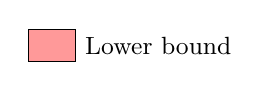
\begin{tikzpicture}[font=\small]
  \begin{scope}[scale=.2]
  \draw[fill=red!40] (0,0) -- (0,2) -- (3,2) --node[anchor=west]{Lower bound} (3,0) -- cycle;
  \end{scope}
  \end{tikzpicture}
  \hfill
  \begin{tikzpicture}[font=\small]
  \begin{scope}[scale=.2]
  \draw[fill=argon orange] (0,0) -- (0,2) -- (3,2) --node[anchor=west]{Solver} (3,0) -- cycle;
  \end{scope}
  \end{tikzpicture}
  \hfill
  \begin{tikzpicture}[font=\small]
  \begin{scope}[scale=.2]
  \draw[fill=argon gray] (0,0) -- (0,2) -- (3,2) --node[anchor=west]{Heuristic} (3,0) -- cycle;
  \end{scope}
  \end{tikzpicture}
}

\mytext[legend.south]{\blockwidth}{anchor = north,
  inner sep = 2pt
}{
  \begin{center}
  \begin{tikzpicture}[font=\scriptsize]

  \pgfplotsset{
    compat=newest,
    xlabel near ticks,
    ylabel near ticks,
  }

  \pgfkeys{/pgf/number format/.cd,
  fixed,
  fixed zerofill,
  precision=0,
  set thousands separator={}}

  \begin{scope}[local bounding box=graph, scale=1.]
    \begin{axis}[
      width=.94\linewidth,
      height=3cm,
      ybar,
      bar width=17pt,
      xlabel={Volatility (in \%)},
      ylabel={Objective value ($\times10^3$)},
      ymin=0,
      ytick=\empty,
      xtick=data,
      axis x line=bottom,
      axis y line=left,
      enlarge x limits=0.2,
      symbolic x coords={$5$,$30$,$50$,$80$},
      %xticklabel style={anchor=base,yshift=-\baselineskip},
      x label style={at={(current axis.right of origin)},anchor=west},
      y label style={at={(current axis.above origin)},rotate=-90,anchor=south},
      nodes near coords={\pgfmathprintnumber\pgfplotspointmeta}
    ]
      \addplot[fill=red!40] coordinates {
        ($5$,746)
        ($30$,828)
        ($50$,921)
        ($80$,1192)
      };
      \addplot[fill=argon orange] coordinates {
        ($5$,967)
        ($30$,1034)
        ($50$,1134)
        ($80$,1381)
      };
      \addplot[fill=argon gray] coordinates {
        ($5$,1176)
        ($30$,1136)
        ($50$,1541)
        ($80$,1640)
      };
    \end{axis}
    \draw (.85\linewidth,1) node[anchor=west]{\large$\servicelvl=70\%$};
  \end{scope}
\end{tikzpicture}


\begin{tikzpicture}[font=\scriptsize]

  \pgfplotsset{
    compat=newest,
    xlabel near ticks,
    ylabel near ticks,
  }

  \pgfkeys{/pgf/number format/.cd,
  fixed,
  fixed zerofill,
  precision=0,
  set thousands separator={}}

  \begin{scope}[local bounding box=graph, scale=1.]
    \begin{axis}[
      width=.94\linewidth,
      height=3cm,
      ybar,
      bar width=17pt,
      xlabel={Volatility (in \%)},
      ylabel={Objective value ($\times10^3$)},
      ymin=0,
      ytick=\empty,
      xtick=data,
      axis x line=bottom,
      axis y line=left,
      enlarge x limits=0.2,
      symbolic x coords={$5$,$30$,$50$,$80$},
      %xticklabel style={anchor=base,yshift=-\baselineskip},
      x label style={at={(current axis.right of origin)},anchor=west},
      y label style={at={(current axis.above origin)},rotate=-90,anchor=south,yshift=4pt},
      nodes near coords={\pgfmathprintnumber\pgfplotspointmeta}
    ]
      \addplot[fill=red!40] coordinates {
        ($5$,813)
        ($30$,895)
        ($50$,1054)
        ($80$,0)
      };
      \addplot[fill=argon orange] coordinates {
        ($5$,957)
        ($30$,1087)
        ($50$,1188)
        ($80$,0)
      };
      \addplot[fill=argon gray] coordinates {
        ($5$,1134)
        ($30$,1112)
        ($50$,1230)
        ($80$,0)
      };
    \end{axis}
    \draw (.85\linewidth,1) node[anchor=west]{\large$\servicelvl=85\%$};
  \end{scope}
\end{tikzpicture}


\begin{tikzpicture}[font=\scriptsize]

  \pgfplotsset{
    compat=newest,
    xlabel near ticks,
    ylabel near ticks,
  }

  \pgfkeys{/pgf/number format/.cd,
  fixed,
  fixed zerofill,
  precision=0,
  set thousands separator={}}

  \begin{scope}[local bounding box=graph, scale=1.]
    \begin{axis}[
      width=.94\linewidth,
      height=3cm,
      ybar,
      bar width=17pt,
      xlabel={Volatility (in \%)},
      ylabel={Objective value ($\times10^3$)},
      ymin=0,
      ytick=\empty,
      xtick=data,
      axis x line=bottom,
      axis y line=left,
      enlarge x limits=0.2,
      symbolic x coords={$5$,$30$,$50$,$80$},
      %xticklabel style={anchor=base,yshift=-\baselineskip},
      x label style={at={(current axis.right of origin)},anchor=west},
      y label style={at={(current axis.above origin)},rotate=-90,anchor=south},
      nodes near coords={\pgfmathprintnumber\pgfplotspointmeta}
    ]
      \addplot[fill=red!40] coordinates {
        ($5$,886)
        ($30$,1173)
        ($50$,1371)
        ($80$,0)
      };
      \addplot[fill=argon orange] coordinates {
        ($5$,956)
        ($30$,1173)
        ($50$,1371)
        ($80$,0)
      };
      \addplot[fill=argon gray] coordinates {
        ($5$,968)
        ($30$,1210)
        ($50$,1396)
        ($80$,0)
      };
    \end{axis}
    \draw (.85\linewidth,1) node[anchor=west]{\large$\servicelvl=95\%$};
  \end{scope}
\end{tikzpicture}



  \end{center}
}

\mytext[8,3.55]{1.8cm}{anchor = south west,
  inner sep = 2pt, fill=white
}{
  \begin{center}
  Infeasible
  \end{center}
}

\mytext[8,1.25]{1.8cm}{anchor = south west,
  inner sep = 2pt, fill=white
}{
  \begin{center}
  Infeasible
  \end{center}
}

\end{myframe}



\begin{myframe}[Results for Lux instances]

\mytext[$(current)+({.505*\blockwidth},0)$]{.95\blockwidth}{anchor = north,
  inner sep = 2pt
}{
  \footnotesize
  \begin{tabular*}{\linewidth}{@{\extracolsep{\fill}}l@{\extracolsep{\fill}}c|@{\extracolsep{\fill}}r|@{\extracolsep{\fill}}r|@{\extracolsep{\fill}}r|@{\extracolsep{\fill}}r|@{\extracolsep{\fill}}l@{\extracolsep{\fill}}}
  & $\beta$ & \multicolumn{4}{c|}{Volatility} & \multicolumn{1}{c}{Output}
  \\
  & & \multicolumn{1}{c|}{5\%} & \multicolumn{1}{c|}{30\%} & \multicolumn{1}{c|}{50\%} & \multicolumn{1}{c|}{80\%} & 
  \\ \hline\hline
  \multirow{9}{*}{\rotatebox{90}{Heuristic}} & 85\% & 1409 & 1516 & 1708 & 1997 & Objective value \hfill {\scriptsize($\times10^3$)}
  \\ \cdashline{3-7}
  &     & 23\% & 21\% & 24\% & 31\% & Multi-sourced items
  \\
  &     & 21\% & 17\% & 20\% & 25\% & (on two plants)
  \\
  &     & 3 & 3 & 3 & 4 & Multi-sourcing (max)
  \\ \cdashline{3-7}
  &     & 24.1\% & 24.7\% & \multicolumn{1}{c|}{--} & \multicolumn{1}{c|}{--} & Gap
  \\
  &     & 1070 & 1142 & \multicolumn{1}{c|}{--} & \multicolumn{1}{c|}{--} & Continuous relaxation \hfill {\scriptsize($\times10^3$)}
  \\
  &     & 8h & 14h & 24h & 24h & Time for bound
  \\ \cdashline{3-7}
  &     & Limit & Yes & Yes & Yes & Feasibility
  \\
  &     & \multicolumn{1}{c|}{--} & 89.4\% & 94.0\% & 94.6\% & Fill rate service level
  \\
  &     & 24h & 1h & 1h & 50min & Evaluation time
  \\ \hline
\end{tabular*}

\begin{itemize}
  \item No results with the LP solver in 24h
  \item[]
  \item Current multi-sourcing in Lux
  \begin{itemize}
    \item Objective value $=6631$
  \end{itemize}
\end{itemize}
}

\mytext[4.3,0.65][text]{\blockwidth}{anchor = south west,
  inner sep = 2pt
}{
  \begin{tikzpicture}[font=\scriptsize]
  \begin{scope}[local bounding box=graph, scale=1.]
    \begin{axis}[width=6cm, height=3cm,
                 %legend entries={2SA-$m$,Det.,Argon},
                 %legend columns={3},
                 %legend cell align={left},
                 % legend style={at={(.5,1)},
                 %               anchor=south,
                 %               font=\scriptsize,
                 %               /tikz/column 2/.style={column sep=8pt,},
                 %               /tikz/column 4/.style={column sep=8pt,},
                 %               /tikz/column 6/.style={column sep=8pt,},
                 % },
                 xtick={2,4,6,8,10}, %xticklabels={2,4,6,8,10},
                 xlabel={Multi-sourcing},
                 every axis x label/.style={ at={(ticklabel* cs:1.05)}, anchor=west, },
                 %xmin=75,
                 %xmax=90,
                 %xmode = log, % logarithmic x axis
                 %ytick={0,20,40,60,80,100}, %yticklabels={1e+06,5e+06,1e+07},
                 ylabel={\% of items}, %scaled y ticks = false, ylabel near ticks,
                 every axis y label/.style={ at={(ticklabel* cs:1.05)}, anchor=east, },
                 ymin=0, ymax=29
                 ]
    \addplot[ybar,fill=argon orange] table [x, y, col sep=comma] {images/current_multi-sourcing.csv};
    \end{axis}
  \end{scope}
\end{tikzpicture}
}

\end{myframe}


\subsection{Conclusion}


\begin{myframe}[Conclusion and perspectives]

\mytext[current][bibliography]{\blockwidth}{anchor = north west,
  inner sep = 2pt
}{
  \begin{itemize}
    \item Conclusion
    \begin{itemize}
      \item We propose a risk constraint to take into account service level
      \item We propose a method to solve it leading to a MIP formulation
      \item We show its efficiency on real dataset
    \end{itemize}
    \item[]
    \item Unpresented works
    \begin{itemize}
      \item Alternative model maximizing service level subject to limited investment
    \end{itemize}
    \item[]
    \item Perspectives
    \begin{itemize}
      \item Decomposition methods (Bender) to solve the MIP
      \item Work on sampling method
    \end{itemize}
  \end{itemize}
}

\end{myframe}


\begin{myframe}[Business context]

\mytext[0,0]{\blockwidth}{anchor = south west,
  inner sep = 0pt
}{
  \begin{tikzpicture}[font=\small]
  
  \pgfmathsetmacro{\timelineup}{5.1}%
  \pgfmathsetmacro{\timelinedown}{4.1}%
  \pgfmathsetmacro{\timelineleft}{0.5}%
  \pgfmathsetmacro{\timelineright}{11.5}%
  \pgfmathsetmacro{\timelinearrow}{0.5}%


  \pgfmathsetmacro{\capacity}{1.75}%
  \pgfmathsetmacro{\multisourcing}{3}%
  \pgfmathsetmacro{\lotsizing}{5}%
  \pgfmathsetmacro{\pdp}{7.5}%
  \pgfmathsetmacro{\scheduling}{10}%


  \pgfmathsetmacro{\legend}{3.25}%


  \begin{scope}[local bounding box=VaR, scale=1.]

  \draw (0,0);

  % Time line
  \shade[left color=argon orange, right color=argon orange!25]
    (\timelineleft,\timelineup) --
    (\timelineright,\timelineup) --
    ({\timelineright+\timelinearrow},{.5*(\timelineup+\timelinedown)}) --
    (\timelineright,\timelinedown) --
    (\timelineleft,\timelinedown) --
    ({\timelineleft+\timelinearrow},{.5*(\timelineup+\timelinedown)}) --
    cycle;
  \draw (\timelineleft,{{.5*(\timelineup+\timelinedown)}}) node[rotate=90, anchor=south]{Long term};
  \draw ({\timelineright+\timelinearrow},{{.5*(\timelineup+\timelinedown)}}) node[rotate=90, anchor=north]{Short term};


  % Decision level
  \draw (\capacity,{.5*(\timelineup+\timelinedown)}) node[anchor=center]{Strategic};
  \draw (\lotsizing,{.5*(\timelineup+\timelinedown)}) node[anchor=center]{\phantom{p}Tactical\phantom{p}};
  \draw (\pdp,{.5*(\timelineup+\timelinedown)}) node[anchor=west]{Operational};
  \draw (\scheduling,{.5*(\timelineup+\timelinedown)}) node[anchor=west]{Real-time\phantom{p}};


  % Capacity-sizing decision
  \draw[-latex] (\capacity,{\timelineup+\legend}) node[anchor=north west, inner sep=2pt]{\textbf{Capacity-sizing}} -- (\capacity,\timelineup);


  % Multi-sourcing decision
  \draw[-latex] (\multisourcing,{\timelinedown-\legend}) node[anchor=south west, inner sep=2pt]{\begin{minipage}{5cm}\begin{tikzpicture}[font=\scriptsize]

\newcommand{\factory}[2][factory]{%
\begin{scope}[shift={(#2)},local bounding box=#1, scale=.4]%
  \draw[line width=1] (0,0) rectangle (2,1.5);%
  \draw (.5,0) rectangle (1,.75) rectangle (1.5,0);%
  \draw[line width=1] (2,0) -- (4,0) -- (4,1.5) -- (3,1) -- (3,1.5) -- (2,1) -- cycle;%
  \draw (2.2,.3) rectangle (2.9,.75);%
  \draw (3.1,.3) rectangle (3.8,.75);%
\end{scope}%
}%


\pgfmathsetmacro{\entrepotright}{3}%
\pgfmathsetmacro{\entrepotleft}{4.6}%
\pgfmathsetmacro{\entrepotheight}{.6}%

\begin{scope}[local bounding box=factory, scale=.7]
  \factory[factoryA]{0,2}
  \factory[factoryB]{0,.5}

  \draw (\entrepotright,2.4) rectangle node[anchor=mid,argon orange]{item A} (\entrepotleft,{2.4+\entrepotheight});
  \draw[-latex, argon orange] ($(factoryA.east)+(.1,.25)$) -- (\entrepotright,{2.4+.5*\entrepotheight});

  \draw (\entrepotright,1.6) rectangle node[anchor=mid,argon orange!50]{item B} (\entrepotleft,{1.6+\entrepotheight});
  \draw[-latex, argon orange!50] ($(factoryA.east)+(.1,0)$) -- (\entrepotright,{1.6+.6*\entrepotheight});
  \draw[-latex, argon orange!50] ($(factoryB.east)+(.1,.25)$) -- (\entrepotright,{1.6+.4*\entrepotheight});

  \draw (\entrepotright,.8) rectangle node[anchor=mid,argon gray!50]{item C} (\entrepotleft,{.8+\entrepotheight});
  \draw[-latex, argon gray!50] ($(factoryA.east)+(.1,-.25)$) -- (\entrepotright,{.8+.6*\entrepotheight});
  \draw[-latex, argon gray!50] ($(factoryB.east)+(.1,0)$) -- (\entrepotright,{.8+.4*\entrepotheight});

  \draw (\entrepotright,0) rectangle node[anchor=mid,argon gray]{item D} (\entrepotleft,{0+\entrepotheight});
  \draw[-latex, argon gray] ($(factoryB.east)+(.1,-.25)$) -- (\entrepotright,{0+.5*\entrepotheight});

\end{scope}

\end{tikzpicture}\\\textbf{Multi-sourcing} (Part \uppercase\expandafter{\romannumeral 3})\end{minipage}} -- (\multisourcing,\timelinedown);


  % Lot-sizing decision
  \draw[-latex] (\lotsizing,{\timelineup+\legend}) node[anchor=north west, inner sep=2pt]{\begin{minipage}{4.5cm}\textbf{Lot-sizing} (Part \uppercase\expandafter{\romannumeral 1})\\\begin{tikzpicture}[font=\footnotesize]

  \begin{scope}[local bounding box=StockLevel, scale=.5]
    % Axe x
    \draw[-angle 60] (-0.2,0) -- (6,0) node[right] {time};
    % Axe y
    \draw[-angle 60] (0,-0.2) -- (0,3) node[anchor=south] {Inventory};

    % Courbe
    \draw[orange, font=\scriptsize, -] (0,0) -- (0,2) --  (2.5,0) -- (2.5,2) -- (5,0) -- (5,2) -- (6,{2-2/2.5});

    \draw[latex-latex] (-.3,0) -- node[sloped,above]{lot} (-.3,2);
    \draw[latex-latex] (0,-.3) -- node[sloped,below]{cover} (2.5,-.3);
  \end{scope}

\end{tikzpicture}
\end{minipage}} -- (\lotsizing,\timelineup);


  % Production planning decision
  \draw[-latex] (\pdp,{\timelinedown-\legend}) node[anchor=south west, inner sep=2pt]{\begin{minipage}{4.5cm}\begin{tikzpicture}[font=\scriptsize]


\pgfmathsetmacro{\week}{.5}%
\pgfmathsetmacro{\weeks}{5}%
\pgfmathsetmacro{\capacity}{1.25}%

\tikzstyle{prodA} = [fill=\maincolor]
\tikzstyle{prodB} = [fill=\maincolor!50]
\tikzstyle{prodC} = [fill=\secondcolor!50]
\tikzstyle{prodD} = [fill=\secondcolor]

\begin{scope}[local bounding box=PDP, scale=1]
  \draw[prodB] (0,0) rectangle (\week,\capacity);
  \draw[prodA] (0,0) rectangle (\week,{.7*\capacity});

  \draw[prodD] ({1*\week},0) rectangle ({2*\week},\capacity);
  \draw[prodC] ({1*\week},0) rectangle ({2*\week},{.6*\capacity});

  \draw[prodC] ({2*\week},0) rectangle ({3*\week},{.9*\capacity});
  \draw[prodA] ({2*\week},0) rectangle ({3*\week},{.3*\capacity});

  \draw[prodB] ({3*\week},0) rectangle ({4*\week},\capacity);
  \draw[prodA] ({3*\week},0) rectangle ({4*\week},{.4*\capacity});

  \draw[prodD] ({4*\week},0) rectangle ({5*\week},{.8*\capacity});
  \draw[prodC] ({4*\week},0) rectangle ({5*\week},{.6*\capacity});

  \foreach \w in {1,2,...,\weeks} \node[anchor=south] (week\w) at ({(\w-.5)*\week},\capacity) {\w};
  \node[anchor=south] (periods) at (week3.north) {Periods};
  \foreach \x in {0,1,...,\weeks} \draw[-] ({\x*\week},0) -- ({\x*\week},\capacity);
  \draw (0,0) rectangle ({\week*\weeks},\capacity);

  \draw[latex-latex] ({-.5*\week},0) -- node[sloped, anchor=south]{Capacity} ({-.5*\week},\capacity);

  \draw[prodD] ({(\weeks+1)*\week},{.125*\capacity}) rectangle node[inner sep=.25cm,anchor=west] {D} ({(\weeks+1.5)*\week},0);
  \draw[prodC] ({(\weeks+1)*\week},{.375*\capacity}) rectangle node[inner sep=.25cm,anchor=west] {C} ({(\weeks+1.5)*\week},{.250*\capacity});
  \draw[prodB] ({(\weeks+1)*\week},{.625*\capacity}) rectangle node[inner sep=.25cm,anchor=west] {B} ({(\weeks+1.5)*\week},{.500*\capacity});
  \draw[prodA] ({(\weeks+1)*\week},{.875*\capacity}) rectangle node[inner sep=.25cm,anchor=west] {A} ({(\weeks+1.5)*\week},{.750*\capacity});
\end{scope}

\end{tikzpicture}\\\textbf{Production planning} (Part \uppercase\expandafter{\romannumeral 2})\end{minipage}} -- (\pdp,\timelinedown);


  % Scheduling decision
  \draw[-latex] (\scheduling,{\timelineup+\legend}) node[anchor=north west, inner sep=2pt]{\textbf{Scheduling}} -- (\scheduling,\timelineup);

  \end{scope}

\end{tikzpicture}

}

\end{myframe}


\section{Continuous-time inventory model (3')}


\begin{myframe}[Continuous-time inventory model (Overview)]

\mytext[current][bibliography]{\blockwidth}{anchor = north west,
  inner sep = 2pt
}{
  \begin{itemize}
    \item Close to \emph{Economic Production Quantity} model but with bound on the number of setups

    \vspace{-.5cm}

    \begin{center}
    \begin{tikzpicture}[font=\footnotesize]

  \newcommand{\longcampain}[3][black]{\draw[#1] (#2,#3) -- ({#2+1.5},{#3+4}) -- ({#2+5.5},#3)}%
 
  \newcommand{\optimalcampain}[3][black]{\draw[#1] (#2,#3) -- ({#2+4/3},{#3+40/15}) -- ({#2+20/3},#3)}%
  \pgfmathsetmacro{\ordinateoptimal}{-13.7}%


  \begin{scope}[local bounding box=VaR, scale=.3]

    % Optimal campain
    \draw[->,argon gray] (-.3,\ordinateoptimal) -- (20,\ordinateoptimal) node[right] {time};
    \draw[->,argon gray] (0,{\ordinateoptimal-.2}) -- (0,{\ordinateoptimal+4.5}) node[above, anchor=south] {inventory};

    \foreach \x in {0,6.666666,...,15} \optimalcampain[argon gray]{\x}{\ordinateoptimal};

    \draw[white] (5.5,\ordinateoptimal) -- node[midway, anchor=south, argon orange, sloped]{$\rate_i-\demand_i$} (7,{\ordinateoptimal+4}) -- node[midway, anchor=south, argon orange, sloped]{$\demand_i$} (11,\ordinateoptimal);

    \foreach \x in {0,5.5,...,16} \longcampain[argon orange]{\x}{\ordinateoptimal};
    \draw[argon orange] (16.5,\ordinateoptimal) -- ({16.5+1.5},{\ordinateoptimal+4}) -- (20,{\ordinateoptimal+2});

    \draw[latex-latex, argon orange] (5.5,{\ordinateoptimal-.5}) -- node[midway, anchor=north]{cover-size $\cover_i$} (11,{\ordinateoptimal-.5});

    \draw[dashed, argon gray!75] (0,{\ordinateoptimal}) -- (0,{\ordinateoptimal-2});
    \draw[dashed, argon gray!75] (18,{\ordinateoptimal}) -- (18,{\ordinateoptimal-2});
    \draw[latex-latex] (0,{\ordinateoptimal-2}) -- node[midway, anchor=north]{$N$ setups} (18,{\ordinateoptimal-2});

  \end{scope}
  
\end{tikzpicture}

    \end{center}

    \vspace{-.5cm}

    \item Closed-form formula in deterministic and stochastic cases

    \vspace{-.25cm}

    $$\mbox{\small$\cover_i^*= \frac{\sum_{j\in\REF}\sqrt{\holding_j\demand_j\bracket{1-\frac{\demand_j}{\rate_j}}}}{\nbsetups\sqrt{\holding_i\demand_i\bracket{1-\frac{\demand_i}{\rate_i}}}}\qquad\forall i\in\REF$}$$

    \vspace{-.25cm}

    \item Extension to multi-line case
    \begin{itemize}
      \item Minimization of a concave function over a polyhedron
    \end{itemize}
  \end{itemize}
}


\end{myframe}


\begin{myframe}[]

\mytext[0,5]{\blockwidth}{anchor = west,
  inner sep = 2pt
}{
  \begin{center}
    \Huge \textcolor{argon orange}{Thank you for your attention!}
  \end{center}
}

\end{myframe}


\addtocounter{framenumber}{-1}


\begin{myframe}[Bibliography]

\mytext[current][bibliography]{\blockwidth}{anchor = north west,
  inner sep = 2pt
}{
  % La bibliographie
  \bibliographystyle{apalike}
  \bibliography{template_diapo}
}

\end{myframe}


\end{document}